\chapter{扩散方程}
\label{chap:diffusion-equations}

把一根细铁棒的中段烧热，再放到隔热的架子上。峰顶很快降下去，两侧慢慢热起来，几分钟之后整根棒几乎同样温度。如果把两端插进冰水，结局又不一样：热量不断从两端流走，棒最后回到冰水的温度。这两个过程遵循同一条局部规律，每一点的温度都在向邻居的平均值靠拢，差别只来自端点。

这条规律能回答的问题比“温度怎样变化”更具体。一个任意形状的鼓包，能不能拆成若干互不干扰、各自衰减的形状？如果棒无限长，一点上的热量过了时间$t$散布成什么样子？初始温度有跳跃时，方程在初始时刻是什么意思？持续加热、端点温度随时间变化时，解又怎样写？

具体的解写出来之后，还要问哪些事情不需要公式也能断定：总热量怎样变，最高温能不能升高，温度的起伏被抹平得多快，粗糙的初值过了片刻会变得多光滑。这些估计同时给出唯一性和对数据的连续依赖，而且把条件暴露得很清楚，有界区域上成立的结论，到了无穷远可能失败。

全章以$(0,1)$上的三角形鼓包为贯穿例子。我们先用方程的局部推导和两类端点确定问题，再分别在有界区间和全空间求解，把持续热源和非零边值叠加进来，然后研究质量、极值、能量和光滑性。最后把“从时刻$0$走到时刻$t$”看成一个算子，并反过来问能否由终态恢复初态：向前平滑得越好，向后恢复就越困难。

\section{初边值问题}
\label{sec:heat-ibvp}

取一根长度为$1$的细棒，中点加热到$1/2$度，向两端线性降到$0$度，初始温度就是一个三角形鼓包
\begin{equation}
 u_0(x)=\min\{x,1-x\},\qquad 0\leq x\leq 1 .
 \label{eq:heat-tent}
\end{equation}
棒的侧面包着隔热层，只有两端可能与外界交换热量。松手之后温度怎样变化？回答它需要一个方程，还需要说清初始时刻和两端发生了什么。

\paragraph{局部守恒与Fourier定律}
先看棒上任意一段$[a,b]$。记$u(x,t)$为温度，选取单位，使单位长度的棒升高一度所需的热量为$1$，于是这一段含有的热量是$\int_a^bu\,\mathrm{d}x$。再记$q(x,t)$为单位时间向右穿过截面$x$的热量，$f(x,t)$为单位长度、单位时间内产生的热量。

如图~\ref{fig:heat-bar-balance}，这一段热量的变化只有三个来源：从左端流入，从右端流出，内部产生。写成等式是
\[
 \frac{\mathrm{d}}{\mathrm{d}t}\int_a^bu\,\mathrm{d}x=q(a,t)-q(b,t)+\int_a^bf\,\mathrm{d}x .
\]

\begin{BookInlineFigure}
  \centering
  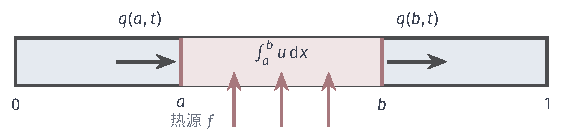
\includegraphics[width=96mm]{figures/06-differential-equations/02-partial-differential-equations/tikz/heat-bar-balance/figure.pdf}
  \caption{细棒上一段$[a,b]$（红色浅底）的热量收支。左右两个箭头是穿过截面的热流$q$，向右为正；下方红色箭头是内部热源$f$。段内热量的变化率等于流入减流出再加内部产生。}
  \label{fig:heat-bar-balance}
\end{BookInlineFigure}

这个等式对任何传递机制都成立，它有$u$和$q$两个未知量，还不能决定演化。补上的一条是物质的性质：热量从高温流向低温，流量正比于温度的斜率，这称为\term{Fourier定律}（Fourier's law）：
\[
 q=-\kappa\,\partial_xu ,
\]
其中$\kappa>0$是导热能力。斜率为正时右边更热，$q<0$，热量向左流，符号正好如此。

设$u$足够光滑。由微积分基本定理，$q(a,t)-q(b,t)=-\int_a^b\partial_xq\,\mathrm{d}x$。把它和Fourier定律代入收支等式，并把对$t$的导数移进积分，得到
\[
 \int_a^b\bigl(\partial_tu-\kappa\,\partial_x^2u-f\bigr)\,\mathrm{d}x=0 .
\]
这对每一段$[a,b]$都成立。被积函数连续，若它在某点不为零，就在一小段上保持同号，取这一小段作$[a,b]$，积分不为零，矛盾。所以被积函数处处为零，即
\begin{equation}
 \partial_tu=\kappa\,\partial_x^2u+f .
 \label{eq:heat-1d-kappa}
\end{equation}
这就是\term{扩散方程}（diffusion equation），在温度的语境下称为\term{热方程}（heat equation）。

\paragraph{向邻居的平均值靠拢}
二阶导数比较的是一点与邻点的平均。由Taylor展开，
\[
 \partial_x^2u(x,t)\approx\frac{2}{h^2}\Bigl(\frac{u(x-h,t)+u(x+h,t)}{2}-u(x,t)\Bigr) .
\]
于是无源时，每一点的温度变化率正比于“邻居平均值减自己”。比邻居平均值高的地方降温，低的地方升温，这就是抹平。

拿式~\eqref{eq:heat-tent}的三角形来看。在两条直线段上，邻居的平均值恰好等于自己，这些点一开始不想变化；只有中点比邻居的平均值高，所以降温从峰顶开始，再逐渐向两侧传开。下面图~\ref{fig:heat-bump-two-boundaries}中最浅的一条曲线正是这样：直线段的大部分还贴着初值，峰顶已经被削圆。

\paragraph{尺度与多维形式}
系数$\kappa$和棒长都可以通过选单位消去。设棒长为$L$，令$x=Ly$、$t=(L^2/\kappa)s$，代入无源方程，得到$\partial_su=\partial_y^2u$。所以时间的自然单位是$L^2/\kappa$：棒长加倍，抹平到同样程度要四倍的时间。这个平方关系后面还会以$\sqrt{t}$的形式反复出现。

高维的推导相同，把截面换成任意小区域的边界，用散度定理把边界通量变成体积分。材料各向异性时通量是$-\bm{A}(\bm{x})\nabla u$，方程是$\partial_tu=\nabla\cdot(\bm{A}\nabla u)+f$，其中$\bm{A}$对称且一致正定。本章取$\bm{A}=\bm{I}$，一维时即$\kappa=1$，这样可以把全部注意力放在解的结构上。

\paragraph{初值、热源与边界}
一个方程不足以确定温度，还要指定开始时的状态和区域边缘的情况。下面把问题写完整，$\Omega\subset\mathbb{R}^{d}$是有界开集，$T>0$。

\begin{definition}[初边值问题]
\label{def:heat-ibvp}
给定源项$f$、初值$u_0$和边界数据$g$，扩散方程的\term{初边值问题}（initial-boundary value problem）是求$u(\bm{x},t)$，使得
\begin{equation}
 \begin{aligned}
  \partial_tu&=\Delta u+f, && \bm{x}\in\Omega,\ 0<t\leq T,\\
  u(\bm{x},0)&=u_0(\bm{x}), && \bm{x}\in\Omega,
 \end{aligned}
 \label{eq:heat-ibvp}
\end{equation}
并在$\partial\Omega\times(0,T]$上满足Dirichlet条件$u=g$或Neumann条件$\partial_{\bm{n}}u=g$。若$\partial_tu$与二阶空间偏导在$\Omega\times(0,T]$上连续，$u$在$\overline\Omega\times[0,T]$上连续，式~\eqref{eq:heat-ibvp}和边界条件逐点成立，就称$u$是\term{经典解}（classical solution）；Neumann情形还要求法向导数在$\partial\Omega\times(0,T]$上存在且连续。
\end{definition}

三种数据各管一件事。初值$u_0$给出出发的状态。方程对时间只有一阶，$\partial_tu$已经由当前的温度分布决定，所以只需要一个初始函数，不必另给初始变化率。源项$f$是持续注入或抽走的热量，$f>0$时加热。边界条件规定外界怎样与区域交换热量。

这些数据在初始时刻的边界上相遇。Dirichlet情形要让$u$在角点连续，必须有$u_0=g(\cdot,0)$，否则解只能在较弱的意义下取得初值；三角形鼓包和零边值满足这一要求。Neumann情形的定义只要求$u$本身连续，式~\eqref{eq:heat-tent}的斜率在端点是$\pm1$，零通量条件要求斜率为$0$，两者不相容，解在角点仍连续，只是空间导数在那里不连续。

\paragraph{固定温度与无通量}
两种齐次边界条件写出来只差一个导数记号，物理含义却完全不同。图~\ref{fig:heat-boundary-meaning}(a)的端点接着大量冰水，温度被钉在$0$，冰水愿意吸收多少热量都可以，通量由解自己决定。图~\ref{fig:heat-boundary-meaning}(b)的端点包着隔热层，通量被规定为零，端点的温度由解自己决定。

\begin{BookInlineFigure}
  \centering
  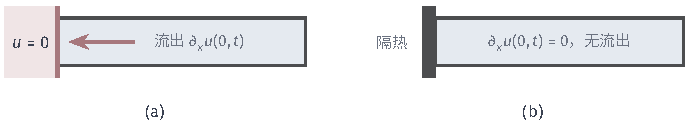
\includegraphics[width=112mm]{figures/06-differential-equations/02-partial-differential-equations/tikz/heat-boundary-meaning/figure.pdf}
  \caption{同一根暖棒左端的两种边界。(a)Dirichlet：端点接冰水，温度固定为$0$，红色箭头表示热量流出，流出率是$\partial_xu(0,t)$，由解决定。(b)Neumann：端点隔热（深灰），通量为零，温度由解决定。}
  \label{fig:heat-boundary-meaning}
\end{BookInlineFigure}

外法向通量是$-\partial_{\bm{n}}u$。所以Neumann数据$\partial_{\bm{n}}u=g>0$表示热量从外面进来，不是流出去。对无源的方程在$(0,1)$上积分，再用微积分基本定理，得到
\[
 \frac{\mathrm{d}}{\mathrm{d}t}\int_0^1u\,\mathrm{d}x=\partial_xu(1,t)-\partial_xu(0,t) .
\]
隔热时右端为零，总热量不变。接冰水时，只要棒内温度为正，左端斜率为正、右端斜率为负，右端小于零，总热量持续减少。

图~\ref{fig:heat-bump-two-boundaries}是同一个三角形在两种边界下的演化，公式下一节推出。短时间内两者几乎一样，因为中段还没有“听到”端点的消息。随后分歧变大：接冰水的鼓包整体下沉到零，隔热的鼓包摊平到平均温度$1/4$。

\begin{BookInlineFigure}
  \centering
  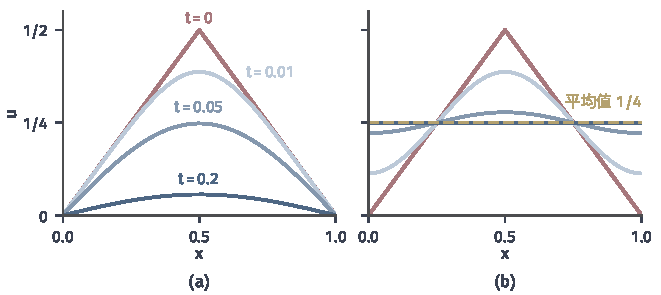
\includegraphics[width=112mm]{figures/06-differential-equations/02-partial-differential-equations/matplotlib/heat-bump-two-boundaries/figure.pdf}
  \caption{三角形初值（红）的演化，蓝色由浅到深为$t=0.01,0.05,0.2$。(a)两端$u=0$。(b)两端$\partial_xu=0$，黄色虚线是初值的平均值$1/4$，$t=0.2$的曲线已与它重合。}
  \label{fig:heat-bump-two-boundaries}
\end{BookInlineFigure}

图~\ref{fig:heat-spacetime-boundaries}把同样的解画在时空平面上。左图的红色竖边表示温度被固定，颜色向上逐渐褪成白色；右图的虚线竖边表示绝热，颜色褪成均匀的浅蓝，总量保留了下来。

\begin{BookInlineFigure}
  \centering
  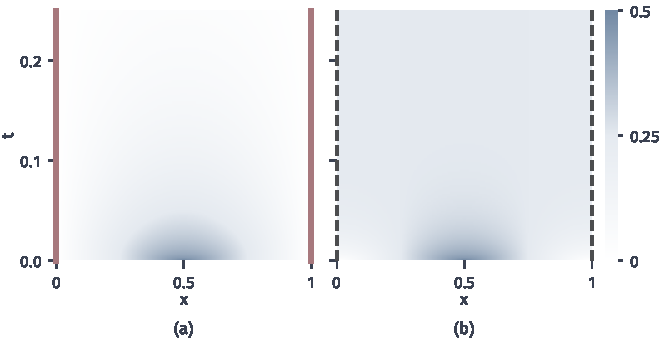
\includegraphics[width=112mm]{figures/06-differential-equations/02-partial-differential-equations/matplotlib/heat-spacetime-boundaries/figure.pdf}
  \caption{三角形初值解的时空温度图，颜色由白到蓝表示温度由$0$到$0.5$，两图色阶相同。(a)两端固定为$0$（红边）。(b)两端无通量（深灰虚边）。}
  \label{fig:heat-spacetime-boundaries}
\end{BookInlineFigure}

把两种条件并列，见表~\ref{tab:heat-boundary-compare}。此外还有介于两者之间的Robin条件$\partial_{\bm{n}}u+\beta u=0$（$\beta>0$），它说流出量正比于端点与环境的温差；$\beta\to0$接近隔热，$\beta\to\infty$接近固定温度。

\begin{BookInlineTable}
  \centering
  \caption{两种齐次边界条件的比较，数值取自三角形初值，$t=0.1$。}
  \label{tab:heat-boundary-compare}
  \begin{tabular}{lll}
    \toprule
    & 固定温度$u=0$ & 无通量$\partial_{\bm{n}}u=0$\\
    \midrule
    规定的量 & 端点温度 & 端点通量\\
    由解决定的量 & 端点通量 & 端点温度\\
    无源时总热量 & 减少 & 不变\\
    $t=0.1$的总热量 & $0.0962$ & $0.2500$\\
    $t=0.1$的中点温度 & $0.1511$ & $0.2539$\\
    \bottomrule
  \end{tabular}
\end{BookInlineTable}


\section{边界模式}
\label{sec:heat-modes}

三角形的形状一直在变，直接跟踪它并不方便。换一个问法：有没有这样的初始形状，演化时形状不变，只是整体按比例缩小？如果有足够多这样的形状，任何初值都可以拆开，各部分分别衰减，再加回去。

\paragraph{离散后的特征向量}
把棒离散成向量，问题就是我们熟悉的。取步长$h=1/4$，内部三个格点$x_j=j/4$，端点取零，用二阶差商代替$\partial_x^2u$，记$\bm{u}(t)$为三个格点上的温度。方程成为线性常微分方程组
\[
 \dot{\bm{u}}=-\bm{K}\bm{u},\qquad
 \bm{K}=16\begin{bmatrix}2&-1&0\\-1&2&-1\\0&-1&2\end{bmatrix} .
\]
矩阵的特征向量正是“形状不变”的初值：若$\bm{K}\bm{v}=\mu\bm{v}$，从$\bm{v}$出发的解是$\mathrm{e}^{-\mu t}\bm{v}$。

三个特征值和特征向量可以手算验证。取$\bm{v}=(\sqrt2/2,\,1,\,\sqrt2/2)^{\top}$，第一行给出$16(\sqrt2-1)\approx6.627$，第二行给出$16(2-\sqrt2)\approx9.373$，比值都是$9.373$，这就是$\mu_1$。全部结果是
\[
 \mu_1=16(2-\sqrt2)\approx9.37,\quad \mu_2=32,\quad \mu_3=16(2+\sqrt2)\approx54.63 .
\]
特征向量恰好是$\sin(k\pi x)$在格点上的取值，$k=1,2,3$，见图~\ref{fig:heat-discrete-modes}。这提示连续问题的“特征向量”是正弦函数，对应的$\mu_k$则应当逼近某个随$k$增长的数。

\begin{BookInlineFigure}
  \centering
  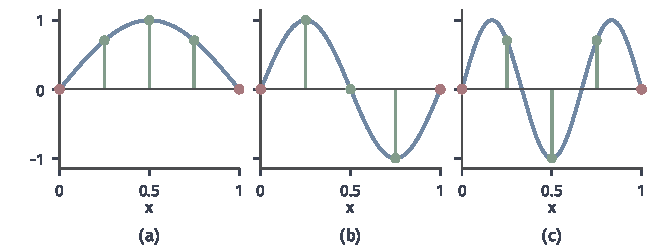
\includegraphics[width=112mm]{figures/06-differential-equations/02-partial-differential-equations/matplotlib/heat-discrete-modes/figure.pdf}
  \caption{三个内部格点的离散问题。绿色竖线是矩阵$\bm{K}$的三个特征向量，蓝线是$\sin(k\pi x)$，红点是固定为零的端点。(a)$k=1$。(b)$k=2$。(c)$k=3$。}
  \label{fig:heat-discrete-modes}
\end{BookInlineFigure}

\paragraph{分离变量}
现在回到连续问题，令$f=0$，寻找形如$u(x,t)=\varphi(x)a(t)$的解，这种做法称为\term{分离变量}（separation of variables）。代入$\partial_tu=\partial_x^2u$，得到
\[
 \varphi(x)\,a'(t)=\varphi''(x)\,a(t) .
\]
在$\varphi$和$a$不为零的地方两边相除，
\[
 \frac{a'(t)}{a(t)}=\frac{\varphi''(x)}{\varphi(x)} .
\]
左边只依赖$t$，右边只依赖$x$，二者相等只能都是常数，记作$-\lambda$。于是偏微分方程分成两个常微分方程：
\begin{equation}
 a'=-\lambda a,\qquad -\varphi''=\lambda\varphi .
 \label{eq:heat-separated}
\end{equation}

时间方程的解是$a(t)=a(0)\mathrm{e}^{-\lambda t}$。空间方程加上边界条件，只对某些$\lambda$有非零解，这称为\term{边界特征值问题}（boundary eigenvalue problem）。边界条件正是在这里进入：它决定哪些形状可用。

\paragraph{Dirichlet边界的模式}
要求$\varphi(0)=\varphi(1)=0$，按$\lambda$的符号分三种情形。

若$\lambda<0$，记$\omega=\sqrt{-\lambda}$，通解是$\varphi=A\cosh\omega x+B\sinh\omega x$。由$\varphi(0)=0$得$A=0$，由$\varphi(1)=B\sinh\omega=0$得$B=0$，没有非零解。

若$\lambda=0$，通解是$\varphi=A+Bx$，两个端点条件同样迫使$A=B=0$。

若$\lambda>0$，记$\omega=\sqrt\lambda$，通解是$\varphi=A\cos\omega x+B\sin\omega x$。由$\varphi(0)=0$得$A=0$。要有非零解，必须$\sin\omega=0$，即$\omega=k\pi$。把振幅归一化后，全部模式是
\begin{equation}
 e_k(x)=\sqrt2\sin(k\pi x),\qquad \lambda_k=k^2\pi^2,\qquad k=1,2,\ldots .
 \label{eq:heat-dirichlet-modes}
\end{equation}

与离散结果比较，连续问题的前三个特征值是
\[
 \lambda_1\approx9.87,\quad \lambda_2\approx39.5,\quad \lambda_3\approx88.8 .
\]
低频的$\mu_1$已经接近$\lambda_1$，高频差别较大，三个格点本来就表示不好高频。

每个模式独立地按$\mathrm{e}^{-k^2\pi^2t}$衰减，频率越高衰减越快。振幅减半的时间是$\ln2/\lambda_k$：$k=1$时约$0.0702$，$k=3$时约$0.0078$，相差九倍。原因就是前面的邻居平均：振荡越快，峰与邻居的落差相对越大。图~\ref{fig:heat-mode-decay}(a)的初值是$\sin(\pi x)+\tfrac12\sin(4\pi x)$，小起伏很快消失，大的拱形缓慢下降；图~\ref{fig:heat-mode-decay}(b)在对数坐标中把衰减画成直线，斜率是$-\lambda_k$。

\begin{BookInlineFigure}
  \centering
  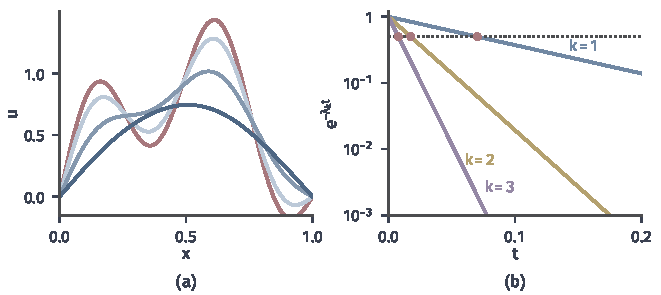
\includegraphics[width=112mm]{figures/06-differential-equations/02-partial-differential-equations/matplotlib/heat-mode-decay/figure.pdf}
  \caption{模式衰减。(a)初值$\sin(\pi x)+\tfrac12\sin(4\pi x)$（红）与$t=0.002,0.008,0.03$的解（蓝色由浅到深）。(b)$k=1,2,3$的振幅因子，纵轴为对数刻度，红点是振幅减半的时刻，虚线高度为$1/2$。}
  \label{fig:heat-mode-decay}
\end{BookInlineFigure}

\paragraph{Neumann边界的模式}
把边界换成$\varphi'(0)=\varphi'(1)=0$，计算只有一处结果不同。$\lambda<0$时，$\varphi'=\omega(A\sinh\omega x+B\cosh\omega x)$，由$\varphi'(0)=0$得$B=0$，由$\varphi'(1)=0$得$A=0$，仍无非零解。$\lambda>0$时，由$\varphi'(0)=0$得$B=0$，再由$\sin\omega=0$得$\omega=k\pi$。

不同的是$\lambda=0$：$\varphi=A+Bx$的导数是$B$，只要$B=0$就满足两个条件，常数活了下来。全部模式是
\begin{equation}
 \tilde{e}_0(x)=1,\quad\lambda_0=0;\qquad \tilde{e}_k(x)=\sqrt2\cos(k\pi x),\quad\lambda_k=k^2\pi^2\quad(k\geq1) .
 \label{eq:heat-neumann-modes}
\end{equation}

$\lambda_0=0$的模式称为\term{零模式}（zero mode），它的时间因子恒为$1$，永远保留。常数没有曲率，每一点都等于邻居的平均值，没有理由变化。这与表~\ref{tab:heat-boundary-compare}的总热量守恒相合：隔热棒里的热量无处可去，它最后全部留在这个常数里。

\paragraph{初值如何确定系数}
要用这些模式表示一般的初值，需要两件事：模式彼此正交，模式足够多。正交性可以直接算。对$j\neq k$，由积化和差，
\[
 \int_0^12\sin(j\pi x)\sin(k\pi x)\,\mathrm{d}x
 =\int_0^1\bigl(\cos((j-k)\pi x)-\cos((j+k)\pi x)\bigr)\,\mathrm{d}x=0 ,
\]
$j=k$时同样的式子给出$1$。

完备性来自Fourier级数：把$(0,1)$上的函数奇延拓到$(-1,1)$，再按周期$2$展开，余弦系数全为零，只剩$\sin(k\pi x)$；偶延拓则只剩余弦。所以$\{e_k\}_{k\geq1}$与$\{\tilde{e}_k\}_{k\geq0}$都是$L^2(0,1)$的标准正交基，三角系统的完备性可参考\BookChapterRef{chap:fourier-transform}{卷四第14章“Fourier变换”}。

于是对$u_0\in L^2(0,1)$，令$c_k=\langle u_0,e_k\rangle$，就有$u_0=\sum_kc_ke_k$（在$L^2$中收敛）和Parseval等式$\sum_kc_k^2=\lVert u_0\rVert_2^2$。把每一项换成衰减后的形式，就得到候选解。它是否真的是解，初值在什么意义下恢复，需要证明。

\begin{theorem}[区间上的模式解]
\label{thm:heat-series}
设$u_0\in L^2(0,1)$，$c_k=\langle u_0,e_k\rangle$，$\lambda_k=k^2\pi^2$，令
\begin{equation}
 u(x,t)=\sum_{k\geq1}c_k\mathrm{e}^{-\lambda_kt}e_k(x) .
 \label{eq:heat-sine-solution}
\end{equation}
则下列结论成立。
\begin{enumerate}
 \item 对每个$t\geq0$，级数在$L^2(0,1)$中收敛，满足
 \begin{equation}
  \lVert u(\cdot,t)\rVert_2\leq\mathrm{e}^{-\pi^2t}\lVert u_0\rVert_2,
  \label{eq:heat-series-decay}
 \end{equation}
 并且$t\to0^+$时$\lVert u(\cdot,t)-u_0\rVert_2\to0$。
 \item 级数及其任意阶逐项导数在$[0,1]\times[t_0,\infty)$上一致收敛（$t_0>0$），所以$u$在$[0,1]\times(0,\infty)$上无穷次可微，逐点满足热方程和零边值。
 \item 若$u_0$连续、分段连续可微且$u_0(0)=u_0(1)=0$，则$\sum_k\lvert c_k\rvert<\infty$，$u$在$[0,1]\times[0,\infty)$上连续，$u(\cdot,0)=u_0$处处成立，$u$是定义~\ref{def:heat-ibvp}意义下的经典解。
\end{enumerate}
\end{theorem}

\begin{proof}
(1)由Parseval等式，系数$c_k\mathrm{e}^{-\lambda_kt}$平方可和，级数收敛。又$\lambda_k\geq\pi^2$，所以
\[
 \lVert u(\cdot,t)\rVert_2^2=\sum_kc_k^2\mathrm{e}^{-2\lambda_kt}\leq\mathrm{e}^{-2\pi^2t}\sum_kc_k^2 .
\]
这就是式~\eqref{eq:heat-series-decay}。初值的恢复同样按坐标计算：
\[
 \lVert u(\cdot,t)-u_0\rVert_2^2=\sum_kc_k^2\bigl(1-\mathrm{e}^{-\lambda_kt}\bigr)^2 .
\]
每一项在$t\to0^+$时趋于零，且不超过可和的$c_k^2$，由级数的控制收敛定理，和趋于零。

(2)由Parseval等式，$\lvert c_k\rvert\leq\lVert u_0\rVert_2$。对$x$求$m$次、对$t$求$n$次后，第$k$项在$t\geq t_0$上的绝对值不超过
\[
 \sqrt2\,\lVert u_0\rVert_2\,(k\pi)^{m+2n}\,\mathrm{e}^{-k^2\pi^2t_0} .
\]
指数因子比$k$的任何幂衰减得都快，这个上界关于$k$可和。由Weierstrass判别法，各阶导数的级数一致收敛，可以逐项求导。每一项都满足方程和零边值，极限也满足。

(3)分部积分一次，边界项因$u_0$在端点为零而消失，得到
\[
 c_k=\frac{1}{k\pi}\int_0^1u_0'(x)\,\sqrt2\cos(k\pi x)\,\mathrm{d}x=\frac{b_k}{k\pi},
\]
其中$b_k$是$u_0'$在标准正交系$\sqrt2\cos(k\pi x)$上的坐标，由Bessel不等式$\sum_kb_k^2\leq\lVert u_0'\rVert_2^2$。再由Cauchy--Schwarz不等式和$\sum_kk^{-2}=\pi^2/6$，
\[
 \sum_k\lvert c_k\rvert\leq\Bigl(\sum_k\frac{1}{k^2\pi^2}\Bigr)^{1/2}\Bigl(\sum_kb_k^2\Bigr)^{1/2}\leq\frac{\lVert u_0'\rVert_2}{\sqrt6} .
\]
于是级数的第$k$项被$\sqrt2\lvert c_k\rvert$一致控制，$u$是连续函数的一致极限，在$[0,1]\times[0,\infty)$上连续。$t=0$时$u(\cdot,0)$连续，又在$L^2$中等于$u_0$，两个连续函数几乎处处相等就处处相等。
\end{proof}

定理的三条分别回答三个问题。第一条对最粗糙的数据也成立，但只说平方积分的距离趋于零，不说每一点的值。第二条说只要过了一点时间，解就无穷光滑，初值有多粗糙无关紧要。第三条说初值和边界相容且有一点光滑性时，一致地恢复。

\begin{example}[三角形的系数]
\label{ex:heat-tent-coefficients}
取式~\eqref{eq:heat-tent}的$u_0$。它连续、分段线性、两端为零，定理~\ref{thm:heat-series}的第三条适用。在$(0,1/2)$上$u_0'=1$，在$(1/2,1)$上$u_0'=-1$，所以
\[
 \int_0^1u_0\sin(k\pi x)\,\mathrm{d}x
 =\frac{1}{k\pi}\Bigl(\int_0^{1/2}\cos(k\pi x)\,\mathrm{d}x-\int_{1/2}^1\cos(k\pi x)\,\mathrm{d}x\Bigr) .
\]
计算两个积分，每一个都贡献$\sin(k\pi/2)/(k\pi)$，于是
\[
 c_k=\frac{2\sqrt2\,\sin(k\pi/2)}{k^2\pi^2} .
\]
偶数$k$的系数为零，这是因为三角形关于中点对称，偶数模式关于中点反对称。前三个非零系数是
\[
 c_1\approx0.2866,\quad c_3\approx-0.0318,\quad c_5\approx0.0115 .
\]
代入式~\eqref{eq:heat-sine-solution}，解是
\[
 u(x,t)=\sum_{k\text{ 奇}}\frac{4\sin(k\pi/2)}{k^2\pi^2}\,\mathrm{e}^{-k^2\pi^2t}\sin(k\pi x) .
\]
\end{example}

在中点，$\sin^2(k\pi/2)=1$，只取第一项得到$\tfrac{4}{\pi^2}\mathrm{e}^{-\pi^2t}$。表~\ref{tab:heat-tent-center}把它与多项求和的结果比较。$t=0$时第一项差得很远，$t=0.1$时已经精确到小数点后三位以上，因为高频项衰减得太快。

\begin{BookInlineTable}
  \centering
  \caption{三角形初值的中点温度$u(1/2,t)$：只取$k=1$一项与级数求和的比较。}
  \label{tab:heat-tent-center}
  \begin{tabular}{lllllll}
    \toprule
    $t$ & $0$ & $0.01$ & $0.02$ & $0.05$ & $0.1$ & $0.2$\\
    \midrule
    第一项 & $0.4053$ & $0.3672$ & $0.3327$ & $0.2474$ & $0.1511$ & $0.0563$\\
    级数 & $0.5000$ & $0.3872$ & $0.3404$ & $0.2480$ & $0.1511$ & $0.0563$\\
    \bottomrule
  \end{tabular}
\end{BookInlineTable}

图~\ref{fig:heat-tent-series}显示了同一件事。图(a)中，$t=0$的系数按$k^{-2}$缓慢下降，时间稍一增加，高频系数就断崖式跌落。图(b)中，初值的折角需要很多项才能描出来；图(c)中，$t=0.02$时一项就很接近真解了。

\begin{BookInlineFigure}
  \centering
  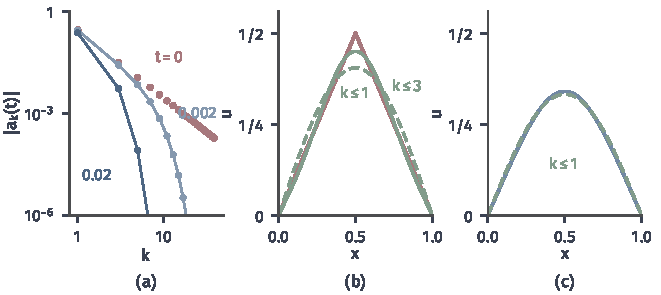
\includegraphics[width=112mm]{figures/06-differential-equations/02-partial-differential-equations/matplotlib/heat-tent-series/figure.pdf}
  \caption{三角形初值的正弦展开。(a)奇数$k$上系数的绝对值$\lvert a_k(t)\rvert=\lvert c_k\rvert\mathrm{e}^{-\lambda_kt}$，红点$t=0$，蓝色点线$t=0.002,0.02$。(b)$t=0$：三角形（红）与$k\leq1$（绿色虚线）、$k\leq3$（绿色实线）的部分和。(c)$t=0.02$：真解（蓝）与$k\leq1$的部分和（绿色虚线）。}
  \label{fig:heat-tent-series}
\end{BookInlineFigure}

\paragraph{Neumann问题与平均值}
余弦基的情形把上面的论证逐字重复，只需注意$\lambda_0=0$。设$u_0\in L^2(0,1)$，$a_0=\int_0^1u_0\,\mathrm{d}x$，$a_k=\langle u_0,\tilde{e}_k\rangle$，解是
\begin{equation}
 u(x,t)=a_0+\sum_{k\geq1}a_k\mathrm{e}^{-k^2\pi^2t}\tilde{e}_k(x) .
 \label{eq:heat-cosine-solution}
\end{equation}
同样的Parseval计算给出
\[
 \lVert u(\cdot,t)-a_0\rVert_2\leq\mathrm{e}^{-\pi^2t}\lVert u_0-a_0\rVert_2 ,
\]
所以温度趋于初值的平均值。

对三角形，$a_0=1/4$。分部积分一次，$\int_0^1u_0\cos(k\pi x)\,\mathrm{d}x$等于$\bigl(2\cos(k\pi/2)-1-(-1)^k\bigr)/(k^2\pi^2)$。只有$k\equiv2\pmod4$时它不为零，等于$-4/(k^2\pi^2)$，于是
\[
 u(x,t)=\frac14-\sum_{k\equiv2\ (\mathrm{mod}\ 4)}\frac{8}{k^2\pi^2}\,\mathrm{e}^{-k^2\pi^2t}\cos(k\pi x) .
\]
最慢的非常数项是$k=2$，衰减率$4\pi^2$，比一般的上界$\pi^2$快。原因仍是对称：$\cos\pi x$关于中点反对称，三角形不含这一分量。例如$t=0.1$时，$\tfrac{2}{\pi^2}\mathrm{e}^{-0.4\pi^2}\approx0.0039$，所以中点温度约$0.2539$，端点温度约$0.2461$，与图~\ref{fig:heat-zero-mode}(a)一致。

\begin{BookInlineFigure}
  \centering
  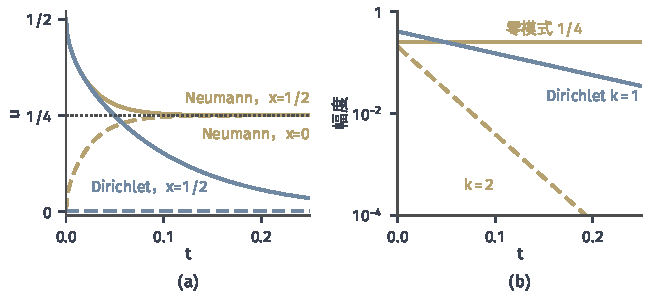
\includegraphics[width=112mm]{figures/06-differential-equations/02-partial-differential-equations/matplotlib/heat-zero-mode/figure.pdf}
  \caption{三角形初值下零模式的作用。(a)中点（实线）与端点（虚线）的温度：Neumann（黄）两条线都趋于$1/4$，Dirichlet（蓝）趋于$0$，蓝色虚线是固定为零的端点。(b)模式幅度，纵轴为对数：Neumann的常数模式$1/4$（黄实线）不变，$k=2$模式幅度$2\pi^{-2}\mathrm{e}^{-4\pi^2t}$（黄虚线）；Dirichlet最低模式幅度$4\pi^{-2}\mathrm{e}^{-\pi^2t}$（蓝）。}
  \label{fig:heat-zero-mode}
\end{BookInlineFigure}

\paragraph{不相容的初值}
定理~\ref{thm:heat-series}第一条的“$L^2$意义下”不是多余的谨慎。取$u_0=1$，两端仍固定为零，初值和边值在角点矛盾。系数是$c_k=\sqrt2(1-(-1)^k)/(k\pi)$，奇数项上为$2\sqrt2/(k\pi)$，于是$\sum_k\lvert c_k\rvert=\infty$，定理的第三条不能用。

$t=0$时部分和在$L^2$中收敛到$1$，但每个部分和在端点都等于$0$，而且靠近端点有固定幅度的过冲，这是\term{Gibbs现象}（Gibbs phenomenon）：奇延拓在端点有高度为$2$的跳跃，部分和的最大值趋于约$1.179$，取$k\leq61$时算得的最大值就是这个数，如图~\ref{fig:heat-corner-layer}(a)。

$t>0$时情形完全改变。定理第二条保证解光滑并且在端点为零，温度在边界附近形成一层过渡，图~\ref{fig:heat-corner-layer}(b)。层的厚度由$\sqrt{t}$决定：把横轴换成$x/(2\sqrt{t})$，不同时刻的层重合到同一条曲线，图~\ref{fig:heat-corner-layer}(c)，这条曲线的公式在下一节得到。

\begin{BookInlineFigure}
  \centering
  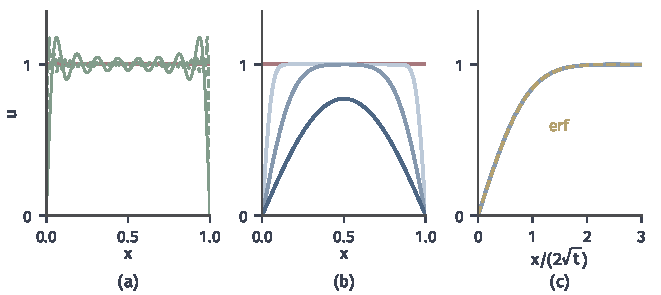
\includegraphics[width=112mm]{figures/06-differential-equations/02-partial-differential-equations/matplotlib/heat-corner-layer/figure.pdf}
  \caption{初值$u_0=1$与零边值不相容。(a)$t=0$：$k\leq15$（绿实线）与$k\leq61$（绿虚线）的部分和在红线附近振荡，端点旁有不随项数消失的过冲。(b)$t=0.001,0.01,0.05$的解（蓝色由浅到深），没有振荡。(c)$t=0.001$、$0.01$的边界层换成变量$x/(2\sqrt{t})$后重合，黄色虚线是$\operatorname{erf}$。}
  \label{fig:heat-corner-layer}
\end{BookInlineFigure}

于是，初值在什么意义下恢复取决于数据：一般的$L^2$初值在$L^2$意义下恢复；连续、分段可微且与边界相容的初值一致地恢复；与边界矛盾的初值在角点附近不可能一致地恢复，但这不妨碍$t>0$时的解是光滑的。


\section{热核}
\label{sec:heat-kernel}

棒无限长时没有端点来挑选模式，频率不再是离散的$k\pi$，而是连成一片。此时局部的一点热量怎样影响后来的场？我们考虑全空间的问题
\begin{equation}
 \partial_tu=\Delta u,\quad \bm{x}\in\mathbb{R}^{d},\ t>0;\qquad u(\bm{x},0)=u_0(\bm{x}) .
 \label{eq:heat-cauchy}
\end{equation}
先用Fourier变换形式地求出公式，再撇开形式推导，直接检验公式在什么条件下给出解、在什么意义下取回初值。

\subsection{核的构造}
\label{sec:heat-kernel-construction}

\paragraph{每个频率一个标量方程}
沿用卷四的约定，Fourier变换写成
\[
 \widehat{u}(\bm{\xi})=\int u(\bm{x})\mathrm{e}^{-2\pi\mathrm{i}\bm{x}\cdot\bm{\xi}}\,\mathrm{d}\bm{x} .
\]
这时对$x_j$求导对应乘以$2\pi\mathrm{i}\xi_j$，Laplace算子对应乘以$-4\pi^2\lvert\bm{\xi}\rvert^2$，这些运算规则都在上一节所引的卷四一章中建立。

设$u$足够好，对式~\eqref{eq:heat-cauchy}关于$\bm{x}$作变换。偏微分方程对每个固定的$\bm{\xi}$变成一个标量常微分方程：
\[
 \partial_t\widehat{u}(\bm{\xi},t)=-4\pi^2\lvert\bm{\xi}\rvert^2\,\widehat{u}(\bm{\xi},t) .
\]
这与上一节的$a'=-\lambda a$完全相同，只是$\lambda$换成了连续变化的$4\pi^2\lvert\bm{\xi}\rvert^2$。解出来是
\begin{equation}
 \widehat{u}(\bm{\xi},t)=\mathrm{e}^{-4\pi^2\lvert\bm{\xi}\rvert^2t}\,\widehat{u}_0(\bm{\xi}) .
 \label{eq:heat-fourier-solution}
\end{equation}
两种模式的对应是精确的：$\sin(k\pi x)=\sin(2\pi(k/2)x)$的频率是$\xi=k/2$，代入$4\pi^2\xi^2$恰好得到$k^2\pi^2$。

\paragraph{乘法还原为卷积}
频域的乘积对应空间的卷积，所以只需找到一个函数，它的变换是$\mathrm{e}^{-4\pi^2\lvert\bm{\xi}\rvert^2t}$。卷四已经算过：$\mathrm{e}^{-\pi\lvert\bm{x}\rvert^2}$的变换是它自身；又把函数$g(\bm{x})$换成$s^{-d}g(\bm{x}/s)$，变换从$\widehat{g}(\bm{\xi})$变成$\widehat{g}(s\bm{\xi})$。

要让指数对上，需要$\pi s^2=4\pi^2t$，即$s=\sqrt{4\pi t}$，这样就得到下面的函数。

\begin{definition}[热核]
\label{def:heat-kernel}
$\mathbb{R}^{d}$上的\term{热核}（heat kernel）是
\begin{equation}
 G(\bm{x},t)=\frac{1}{(4\pi t)^{d/2}}\exp\Bigl(-\frac{\lvert\bm{x}\rvert^2}{4t}\Bigr),\qquad \bm{x}\in\mathbb{R}^{d},\ t>0 .
 \label{eq:heat-kernel}
\end{equation}
对初值$u_0$，定义\term{卷积表示}（convolution representation）
\begin{equation}
 u(\bm{x},t)=\int_{\mathbb{R}^{d}}G(\bm{x}-\bm{y},t)\,u_0(\bm{y})\,\mathrm{d}\bm{y} .
 \label{eq:heat-convolution}
\end{equation}
\end{definition}

到这里的推导要求$u$有变换、能逐点解常微分方程、乘积能还原，都是形式的。下面的做法不再依赖它们，而是直接研究式~\eqref{eq:heat-kernel}和式~\eqref{eq:heat-convolution}。

\begin{theorem}[热核的基本性质]
\label{thm:heat-kernel-properties}
对$t>0$，式~\eqref{eq:heat-kernel}的$G$满足：
\begin{enumerate}
 \item $G>0$，并且$G(\cdot,t)$在$\mathbb{R}^{d}$上的积分等于$1$；
 \item 满足尺度关系
 \begin{equation}
  G(\bm{x},t)=t^{-d/2}G(\bm{x}/\sqrt{t},1) ;
  \label{eq:heat-kernel-scaling}
 \end{equation}
 \item 每个坐标的二阶矩等于$2t$；
 \item 在$\mathbb{R}^{d}\times(0,\infty)$上$\partial_tG=\Delta G$。
\end{enumerate}
\end{theorem}

\begin{proof}
正性由公式可见。积分按坐标分解成$d$个一维积分的乘积。一维情形代换$x=2\sqrt{t}\,z$，
\[
 \int_{\mathbb{R}}\frac{1}{\sqrt{4\pi t}}\mathrm{e}^{-x^2/(4t)}\,\mathrm{d}x=\frac{1}{\sqrt\pi}\int_{\mathbb{R}}\mathrm{e}^{-z^2}\,\mathrm{d}z=1 .
\]
尺度关系由公式直接代入得到。二阶矩中其余坐标积分为$1$，剩下的一维积分用同一代换，再用$\int z^2\mathrm{e}^{-z^2}\,\mathrm{d}z=\sqrt\pi/2$，得到
\[
 \int_{\mathbb{R}}x^2G(x,t)\,\mathrm{d}x=\frac{4t}{\sqrt\pi}\int_{\mathbb{R}}z^2\mathrm{e}^{-z^2}\,\mathrm{d}z=2t .
\]

最后计算导数。令$r=\lvert\bm{x}\rvert$，对$t$求导得到
\[
 \partial_tG=\Bigl(-\frac{d}{2t}+\frac{r^2}{4t^2}\Bigr)G .
\]
对$x_i$求一次导数得$\partial_iG=-\tfrac{x_i}{2t}G$，再求一次并对$i$求和，
\[
 \Delta G=\sum_{i}\Bigl(-\frac{1}{2t}+\frac{x_i^2}{4t^2}\Bigr)G=\Bigl(-\frac{d}{2t}+\frac{r^2}{4t^2}\Bigr)G .
\]
两式相等。
\end{proof}

四条性质各有含义。正性和积分为$1$说卷积是一种加权平均，总热量不变。尺度关系说时间不产生新形状，只把同一个钟形按$\sqrt{t}$拉宽、按$t^{-d/2}$压低。二阶矩说方差随时间线性增长，所以宽度是$\sqrt{2t}$。

具体地，一维时$t=0.01,0.04,0.16$的峰值是$2.82,\,1.41,\,0.705$，标准差是$0.141,\,0.283,\,0.566$：时间变为四倍，宽度加倍，峰值减半，图~\ref{fig:heat-kernel-scaling}。这就是初边值问题里“棒长加倍、时间四倍”的另一面。

\begin{BookInlineFigure}
  \centering
  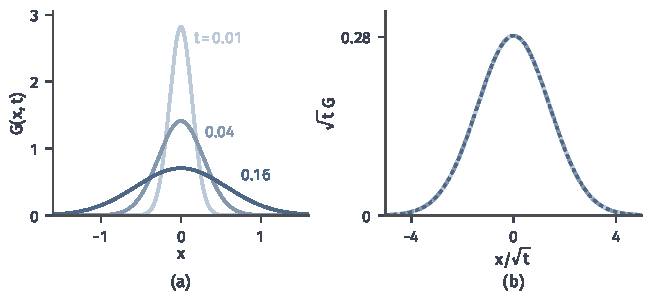
\includegraphics[width=112mm]{figures/06-differential-equations/02-partial-differential-equations/matplotlib/heat-kernel-scaling/figure.pdf}
  \caption{一维热核。(a)$t=0.01,0.04,0.16$时的$G(x,t)$（蓝色由浅到深）。(b)改用尺度化坐标后的$\sqrt{t}\,G$与$x/\sqrt{t}$，三个时刻（实线、虚线、点线）重合到同一条曲线。}
  \label{fig:heat-kernel-scaling}
\end{BookInlineFigure}

\paragraph{卷积是加权平均}
式~\eqref{eq:heat-convolution}的读法是：时刻$t$在$\bm{x}$处的温度，是初值以$\bm{x}$为中心、宽度约$\sqrt{2t}$的Gauss加权平均。也可以反过来读：$\bm{y}$处的一点初始热量$u_0(\bm{y})\,\mathrm{d}\bm{y}$，到时刻$t$散成以$\bm{y}$为中心的钟形，所有钟形叠加成解。

取方框$u_0=\mathbb{I}_{[-1/2,1/2]}$为例。引入误差函数
\[
 \operatorname{erf}(z)=\frac{2}{\sqrt\pi}\int_0^z\mathrm{e}^{-s^2}\,\mathrm{d}s .
\]
一维积分经代换$z=(x-y)/(2\sqrt{t})$化为
\begin{equation}
 u(x,t)=\frac12\Bigl(\operatorname{erf}\frac{x+1/2}{2\sqrt{t}}-\operatorname{erf}\frac{x-1/2}{2\sqrt{t}}\Bigr) .
 \label{eq:heat-box-solution}
\end{equation}

图~\ref{fig:heat-convolution-weights}取$x=0.7$，$t=0.04$。紫色钟形在方框内的部分（蓝色浅底）的面积就是这一点的温度，代入式~\eqref{eq:heat-box-solution}得$0.240$。这一点在方框外，初值为零，可是加权平均已经够到了方框。

\begin{BookInlineFigure}
  \centering
  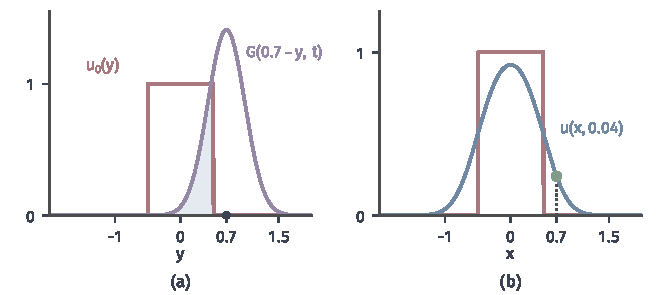
\includegraphics[width=112mm]{figures/06-differential-equations/02-partial-differential-equations/matplotlib/heat-convolution-weights/figure.pdf}
  \caption{卷积作为加权平均。(a)方框初值（红）与以$x=0.7$为中心、$t=0.04$的权重$G(0.7-y,t)$（紫），蓝色浅底的面积等于$u(0.7,0.04)$。(b)解$u(\cdot,0.04)$（蓝），绿点是$x=0.7$处的值$0.240$。}
  \label{fig:heat-convolution-weights}
\end{BookInlineFigure}

\paragraph{传播范围}
热核处处为正，于是只要$u_0\geq0$不恒为零，对任意小的$t>0$，$u$在每一点都严格为正。扰动瞬间到达无穷远，这一性质称为\term{无穷传播速度}（infinite speed of propagation），它与下一章波动方程的有限速度截然不同。

但“到达”的量极小。由式~\eqref{eq:heat-box-solution}，$t=0.01$时距离方框中心$2$的地方温度只有约$1.4\times10^{-26}$，$t=0.1$时距离$3$的地方约$1.1\times10^{-8}$。图~\ref{fig:heat-tails}(a)中尾部在对数坐标下是向下弯的抛物线，这是$\mathrm{e}^{-x^2/(4t)}$的特征。

想知道“热量实际传到哪里”，可以固定一个小的阈值看等值线。图~\ref{fig:heat-tails}(b)是$u=10^{-3}$的位置，它按$\sqrt{t}$前进，早期很快，后来越来越慢，并不是匀速推进的波前。

\begin{BookInlineFigure}
  \centering
  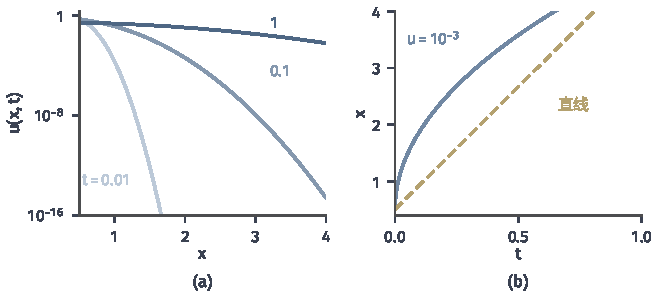
\includegraphics[width=112mm]{figures/06-differential-equations/02-partial-differential-equations/matplotlib/heat-tails/figure.pdf}
  \caption{方框初值的远场。(a)$x>1/2$上的解，纵轴对数，$t=0.01,0.1,1$（蓝色由浅到深）。(b)等值线$u=10^{-3}$的位置（蓝），黄色虚线是连接其起点和终点的直线，匀速前进的前沿应当沿这样的直线。}
  \label{fig:heat-tails}
\end{BookInlineFigure}

这里要说清类比的边界。把热核读成“热量瞬间传到远处”，描述的是这个数学模型。真实的热传递由有限速度的微观运动实现，Fourier定律只是在足够大的尺度上的近似，远处$10^{-26}$量级的温度变化没有物理意义。模型的价值在于$\sqrt{t}$的尺度和被压到极小的尾部，而不在严格的正性上。

\paragraph{频率的衰减}
同一个解也可以在频域读。式~\eqref{eq:heat-fourier-solution}说，频率$\bm{\xi}$的分量乘以$\mathrm{e}^{-4\pi^2\lvert\bm{\xi}\rvert^2t}$。这个因子在$\lvert\bm{\xi}\rvert=1/(2\pi\sqrt{t})$处降到$\mathrm{e}^{-1}$，更高的频率几乎全被抹掉。例如$t=0.01$时$\xi=5$的因子是$\mathrm{e}^{-\pi^2}\approx5\times10^{-5}$。

所以热核是一个低通滤波器，时间越长，通带越窄，图~\ref{fig:heat-fourier-multiplier}。空间和频率的两种读法互为对偶：空间上钟形的宽度按$\sqrt{t}$增长，频率上通带的宽度按$1/\sqrt{t}$收缩。方框的尖角含有缓慢衰减的高频，滤掉之后角就圆了。

\begin{BookInlineFigure}
  \centering
  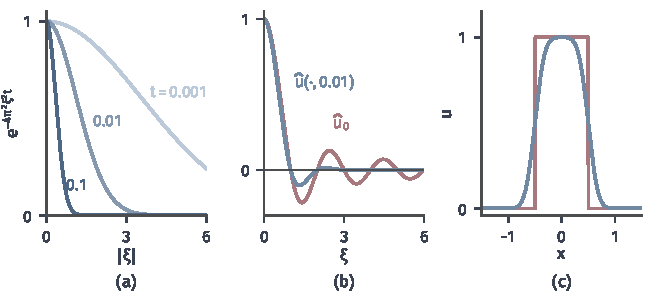
\includegraphics[width=112mm]{figures/06-differential-equations/02-partial-differential-equations/matplotlib/heat-fourier-multiplier/figure.pdf}
  \caption{热传播的频域作用。(a)乘子$\mathrm{e}^{-4\pi^2\xi^2t}$，$t=0.001,0.01,0.1$（蓝色由浅到深）。(b)方框的变换$\widehat{u}_0=\sin(\pi\xi)/(\pi\xi)$（红）与乘上$t=0.01$的乘子后的结果（蓝）。(c)空间中的方框（红）与$t=0.01$的解（蓝）。}
  \label{fig:heat-fourier-multiplier}
\end{BookInlineFigure}

\paragraph{公式何时给出解}
式~\eqref{eq:heat-convolution}的积分未必收敛。$u_0$可以无界，但不能增长得比核衰减得还快。下面的条件恰好刻画这个界线：存在$T>0$，使
\begin{equation}
 \int_{\mathbb{R}^{d}}\lvert u_0(\bm{y})\rvert\,\mathrm{e}^{-\lvert\bm{y}\rvert^2/(4T)}\,\mathrm{d}\bm{y}<\infty .
 \label{eq:heat-integrability}
\end{equation}
有界的可测函数、$L^p$函数（$1\leq p\leq\infty$）都满足它，并且$T$可以取任意正数。

\begin{theorem}[卷积解的可微性]
\label{thm:heat-convolution-smooth}
设$u_0$可测且满足式~\eqref{eq:heat-integrability}。则式~\eqref{eq:heat-convolution}的积分对$\bm{x}\in\mathbb{R}^{d}$、$0<t<T$绝对收敛，$u$在$\mathbb{R}^{d}\times(0,T)$上无穷次可微，且可以在积分号下求导；特别地
\begin{equation}
 \partial_tu=\Delta u,\qquad \bm{x}\in\mathbb{R}^{d},\ 0<t<T .
 \label{eq:heat-convolution-solves}
\end{equation}
\end{theorem}

\begin{proof}
固定紧集$K\subset\mathbb{R}^{d}\times(0,T)$，其上$\lvert\bm{x}\rvert\leq R$，$t_0\leq t\leq t_1<T$。关键是用一个与$(\bm{x},t)$无关的可积函数控制被积函数及其导数。

取$\theta>0$使$(1+\theta)t_1<T$，再取$\sigma\in(0,1)$，使$(1+\theta)t_1/(1-\sigma)\leq T$。由三角不等式和Young不等式，对任意$\bm{x},\bm{y}$，
\[
 \lvert\bm{y}\rvert^2\leq(1+\theta)\lvert\bm{x}-\bm{y}\rvert^2+\bigl(1+\theta^{-1}\bigr)\lvert\bm{x}\rvert^2 .
\]
把它改写成对$\lvert\bm{x}-\bm{y}\rvert^2$的下界，并用$t\leq t_1$，得到
\[
 \frac{(1-\sigma)\lvert\bm{x}-\bm{y}\rvert^2}{4t}\geq\frac{(1-\sigma)\lvert\bm{y}\rvert^2}{4(1+\theta)t_1}-C_1\geq\frac{\lvert\bm{y}\rvert^2}{4T}-C_1 ,
\]
其中常数$C_1$只依赖$R$、$t_0$、$\theta$、$\sigma$。

$G$对$\bm{x}$、$t$的任意阶导数等于$G$乘以一个$\bm{x}$和$1/t$的多项式。在$K$上这个多项式关于$\lvert\bm{x}-\bm{y}\rvert$有多项式增长，而多项式被指数$\mathrm{e}^{-\sigma\lvert\bm{x}-\bm{y}\rvert^2/(4t)}$压住。于是每个导数的绝对值满足
\[
 \bigl\lvert\partial^{\alpha}_{\bm{x}}\partial_t^{n}G(\bm{x}-\bm{y},t)\bigr\rvert\leq C\,\mathrm{e}^{-(1-\sigma)\lvert\bm{x}-\bm{y}\rvert^2/(4t)}\leq C'\,\mathrm{e}^{-\lvert\bm{y}\rvert^2/(4T)} .
\]
乘以$\lvert u_0\rvert$后可积。由控制收敛定理，积分绝对收敛，且可以在积分号下任意次求导。定理~\ref{thm:heat-kernel-properties}的第四条给出式~\eqref{eq:heat-convolution-solves}。
\end{proof}

这个结论里没有要求初值连续，这是扩散的平滑作用的第一次定量出现，后面还要专门研究。条件中的$T$不能随意增大，下面的例子说明它是准确的。

\begin{example}[快速增长的初值]
\label{ex:heat-gaussian-growth}
取$d=1$，$u_0(x)=\mathrm{e}^{ax^2}$，$a>0$。此时式~\eqref{eq:heat-integrability}成立当且仅当$T<1/(4a)$。式~\eqref{eq:heat-convolution}的指数是$y$的二次式，记$p=1/(4t)-a$，当$t<1/(4a)$时$p>0$。把指数写成
\[
 -py^2+\frac{xy}{2t}-\frac{x^2}{4t} .
\]
由Gauss积分
\[
 \int_{\mathbb{R}}\mathrm{e}^{-py^2+by}\,\mathrm{d}y=\sqrt{\frac{\pi}{p}}\,\mathrm{e}^{b^2/(4p)},
\]
取$b=x/(2t)$，振幅因子是$(4\pi t)^{-1/2}\sqrt{\pi/p}$，它等于$(1-4at)^{-1/2}$。指数部分合并后是$ax^2/(1-4at)$，于是
\begin{equation}
 u(x,t)=\frac{1}{\sqrt{1-4at}}\exp\Bigl(\frac{ax^2}{1-4at}\Bigr),\qquad 0\leq t<\frac{1}{4a} .
 \label{eq:heat-gaussian-growth}
\end{equation}
$t\to1/(4a)$时$u(0,t)\to\infty$，解在有限时间爆炸。
\end{example}

图~\ref{fig:heat-growth-limit}取$a=1/2$，由式~\eqref{eq:heat-gaussian-growth}，爆炸时刻是$t=1/2$。这里的爆炸并不违背“热量被抹平”的直觉：无穷远处温度增长得太快，加权平均从远处吸进来的热量越来越多，直到积分发散。

\begin{BookInlineFigure}
  \centering
  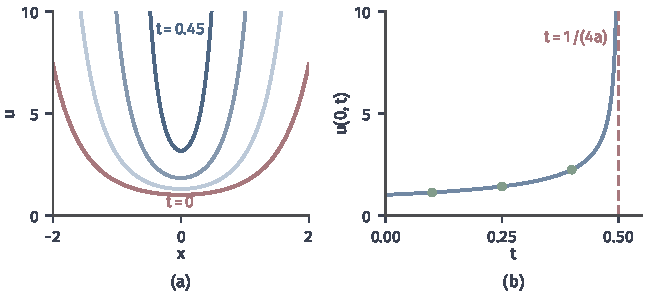
\includegraphics[width=112mm]{figures/06-differential-equations/02-partial-differential-equations/matplotlib/heat-growth-limit/figure.pdf}
  \caption{初值$\mathrm{e}^{x^2/2}$（$a=1/2$）的卷积解。(a)$t=0$（红）与$t=0.2,0.35,0.45$（蓝色由浅到深）。(b)中心温度$u(0,t)=(1-2t)^{-1/2}$（蓝），绿点是直接数值积分的结果，红色虚线是爆炸时刻$t=1/(4a)$。}
  \label{fig:heat-growth-limit}
\end{BookInlineFigure}

\subsection{初值恢复}
\label{sec:heat-recovery}

卷积公式只在$t>0$时有定义，定理~\ref{thm:heat-convolution-smooth}没有提到初值。$t\to0^+$时$u$回到$u_0$吗？答案取决于数据和“回到”的含义。

\paragraph{质量向一点集中}
直观上，$G(\cdot,t)$的总质量始终是$1$，宽度却趋于零，加权平均只看越来越近的邻域，所以应当趋于该点的值。这样的一族函数称为\term{恒同逼近}（approximate identity）。所有证明都用到同一个定量事实：对任意$\delta>0$，由尺度关系~\eqref{eq:heat-kernel-scaling}，
\begin{equation}
 \int_{\lvert\bm{y}\rvert\geq\delta}G(\bm{y},t)\,\mathrm{d}\bm{y}=\int_{\lvert\bm{z}\rvert\geq\delta/\sqrt{t}}G(\bm{z},1)\,\mathrm{d}\bm{z}\ \longrightarrow\ 0,\quad t\to0^+ .
 \label{eq:heat-tail}
\end{equation}
右边是一个可积函数在越来越远的区域上的积分，所以趋于零。图~\ref{fig:heat-approx-identity}显示了$\lvert\bm{y}\rvert\geq\delta$上的尾部质量怎样随$t$变化。

\begin{BookInlineFigure}
  \centering
  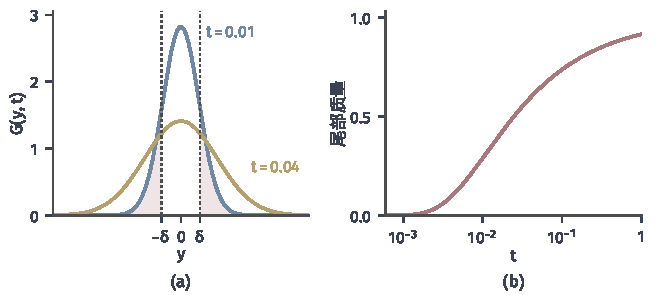
\includegraphics[width=112mm]{figures/06-differential-equations/02-partial-differential-equations/matplotlib/heat-approx-identity/figure.pdf}
  \caption{热核质量的集中。(a)$t=0.01$（蓝）与$t=0.04$（黄）的核，红色浅底是$t=0.01$时$\lvert y\rvert\geq\delta$的尾部，$\delta=0.15$。(b)该尾部质量$\operatorname{erfc}(\delta/(2\sqrt{t}))$随$t$的变化，横轴为对数。}
  \label{fig:heat-approx-identity}
\end{BookInlineFigure}

\paragraph{一致恢复}
记$C_0(\mathbb{R}^{d})$为在无穷远趋于零的连续函数，它们都有界且一致连续，所以只需讨论有界一致连续的函数。一致连续性是这里的关键：同一个$\delta$要对所有的点起作用。

\begin{theorem}[一致范数下的恢复]
\label{thm:heat-uniform-recovery}
设$u_0$在$\mathbb{R}^{d}$上有界且一致连续，特别地可以是$u_0\in C_0(\mathbb{R}^{d})$。则式~\eqref{eq:heat-convolution}给出的$u$满足
\begin{equation}
 \lim_{t\to0^+}\sup_{\bm{x}\in\mathbb{R}^{d}}\lvert u(\bm{x},t)-u_0(\bm{x})\rvert=0 .
 \label{eq:heat-uniform-recovery}
\end{equation}
\end{theorem}

\begin{proof}
因为$G$的积分为$1$，可以把$u_0(\bm{x})$写进积分。再代换$\bm{y}\mapsto\bm{x}-\bm{y}$，
\[
 u(\bm{x},t)-u_0(\bm{x})=\int G(\bm{y},t)\bigl(u_0(\bm{x}-\bm{y})-u_0(\bm{x})\bigr)\,\mathrm{d}\bm{y} .
\]
任取$\varepsilon>0$，由一致连续性取$\delta>0$，使$\lvert\bm{y}\rvert<\delta$时对所有$\bm{x}$都有$\lvert u_0(\bm{x}-\bm{y})-u_0(\bm{x})\rvert<\varepsilon$。

把积分分成$\lvert\bm{y}\rvert<\delta$和$\lvert\bm{y}\rvert\geq\delta$两部分。第一部分不超过$\varepsilon\int G=\varepsilon$。第二部分中被积的差不超过$2\lVert u_0\rVert_\infty$，于是
\[
 \lvert u(\bm{x},t)-u_0(\bm{x})\rvert\leq\varepsilon+2\lVert u_0\rVert_\infty\int_{\lvert\bm{y}\rvert\geq\delta}G(\bm{y},t)\,\mathrm{d}\bm{y} .
\]
右端与$\bm{x}$无关。由式~\eqref{eq:heat-tail}，$t$充分小时第二项小于$\varepsilon$。
\end{proof}

\paragraph{$L^p$恢复}
积分型的范数不需要逐点的连续性，$L^p$函数在平移下的连续性起到一致连续性的作用。

\begin{theorem}[$L^p$范数下的恢复]
\label{thm:heat-lp-recovery}
设$1\leq p<\infty$，$u_0\in L^p(\mathbb{R}^{d})$。则对$t>0$，$u(\cdot,t)\in L^p$，并且
\begin{equation}
 \lVert u(\cdot,t)\rVert_p\leq\lVert u_0\rVert_p,\qquad \lim_{t\to0^+}\lVert u(\cdot,t)-u_0\rVert_p=0 .
 \label{eq:heat-lp-recovery}
\end{equation}
第一个不等式对$p=\infty$也成立。
\end{theorem}

\begin{proof}
记$(\tau_{\bm{y}}u_0)(\bm{x})=u_0(\bm{x}-\bm{y})$。解是平移函数的加权平均：
\[
 u(\cdot,t)=\int G(\bm{y},t)\,\tau_{\bm{y}}u_0\,\mathrm{d}\bm{y} .
\]
积分形式的Minkowski不等式说，平均的范数不超过范数的平均，所以
\[
 \lVert u(\cdot,t)\rVert_p\leq\int G(\bm{y},t)\lVert\tau_{\bm{y}}u_0\rVert_p\,\mathrm{d}\bm{y}=\lVert u_0\rVert_p .
\]
$p=\infty$时这由$\lvert u\rvert\leq\lVert u_0\rVert_\infty\int G$直接得到。

同样地，把$u_0$写进积分后，
\[
 \lVert u(\cdot,t)-u_0\rVert_p\leq\int G(\bm{y},t)\,\lVert\tau_{\bm{y}}u_0-u_0\rVert_p\,\mathrm{d}\bm{y} .
\]
任取$\varepsilon>0$。平移在$L^p$中连续，这要求$p<\infty$，可参考\BookChapterRef{chap:function-approximation}{卷四第20章“函数逼近”}，所以存在$\delta>0$，使$\lvert\bm{y}\rvert<\delta$时$\lVert\tau_{\bm{y}}u_0-u_0\rVert_p<\varepsilon$。

分成$\lvert\bm{y}\rvert<\delta$和$\lvert\bm{y}\rvert\geq\delta$两部分。第一部分不超过$\varepsilon$。第二部分中差的范数不超过$2\lVert u_0\rVert_p$，由式~\eqref{eq:heat-tail}，$t$充分小时小于$\varepsilon$。
\end{proof}

用方框验证收敛的快慢。每条边附近$u-u_0$的绝对值在距边$s$处约为$\tfrac12\operatorname{erfc}(s/(2\sqrt{t}))$，$t$小时两条边互不干扰。边的两侧合起来积分，用$\int_0^\infty\operatorname{erfc}=1/\sqrt\pi$，每条边贡献
\[
 2\int_0^\infty\frac12\operatorname{erfc}\frac{s}{2\sqrt{t}}\,\mathrm{d}s=2\sqrt{\frac{t}{\pi}} ,
\]
所以$\lVert u(\cdot,t)-u_0\rVert_1\approx4\sqrt{t/\pi}$。$t=0.01$时这个数是$0.2257$，数值积分的结果与它一致。

图~\ref{fig:heat-recovery-norms}把几种范数放在一起。方框的$L^1$距离按$t^{1/2}$下降，$L^2$距离按$t^{1/4}$下降，一致距离却始终是$1/2$，因为边界上的解总是取$1/2$，而边的一侧初值是$1$。连续的三角形$\max\{1-\lvert x\rvert,0\}$在一致范数下收敛，折角处的下降是$2\sqrt{t/\pi}$。

\begin{BookInlineFigure}
  \centering
  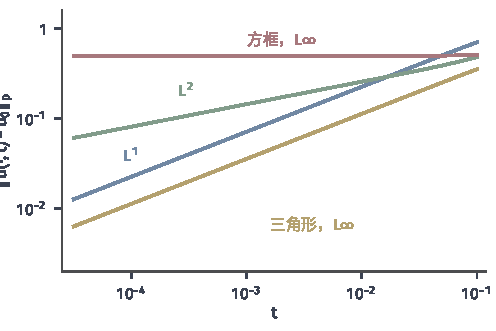
\includegraphics[width=84mm]{figures/06-differential-equations/02-partial-differential-equations/matplotlib/heat-recovery-norms/figure.pdf}
  \caption{解到初值的距离随$t$的变化，双对数坐标。方框初值$\mathbb{I}_{[-1/2,1/2]}$的$L^1$（蓝）、$L^2$（绿）、$L^\infty$（红）距离；连续三角形$\max\{1-\lvert x\rvert,0\}$的$L^\infty$距离（黄）。}
  \label{fig:heat-recovery-norms}
\end{BookInlineFigure}

\paragraph{连续点的恢复}
一般的初值只要在一点连续，解就在这一点取回初值，这是局部的结论，不需要整体的有界性。

\begin{theorem}[连续点的恢复]
\label{thm:heat-pointwise-recovery}
设$u_0$可测且满足式~\eqref{eq:heat-integrability}，在$\bm{x}_0$处连续。则
\begin{equation}
 \lim_{(\bm{x},t)\to(\bm{x}_0,0^+)}u(\bm{x},t)=u_0(\bm{x}_0) .
 \label{eq:heat-pointwise-recovery}
\end{equation}
\end{theorem}

\begin{proof}
仍利用$G$的积分为$1$，写成
\[
 u(\bm{x},t)-u_0(\bm{x}_0)=\int G(\bm{x}-\bm{y},t)\bigl(u_0(\bm{y})-u_0(\bm{x}_0)\bigr)\,\mathrm{d}\bm{y} .
\]
任取$\varepsilon>0$，取$\delta>0$使$\lvert\bm{y}-\bm{x}_0\rvert<\delta$时$\lvert u_0(\bm{y})-u_0(\bm{x}_0)\rvert<\varepsilon$。只考虑$\lvert\bm{x}-\bm{x}_0\rvert<\delta/2$。近处$\lvert\bm{y}-\bm{x}_0\rvert<\delta$的积分不超过$\varepsilon$。

在远处$\lvert\bm{y}-\bm{x}_0\rvert\geq\delta$，有$\lvert\bm{x}-\bm{y}\rvert\geq\delta/2$，并且$\lvert\bm{x}-\bm{y}\rvert$不小于$\lvert\bm{y}-\bm{x}_0\rvert/2$。

把指数平分成两半，一半用第一个下界，另一半用第二个下界：
\[
 \mathrm{e}^{-\lvert\bm{x}-\bm{y}\rvert^2/(4t)}\leq\mathrm{e}^{-\delta^2/(32t)}\,\mathrm{e}^{-\lvert\bm{y}-\bm{x}_0\rvert^2/(32t)} .
\]
限制$t\leq T/16$，并利用
\[
 \lvert\bm{y}-\bm{x}_0\rvert^2\geq\frac12\lvert\bm{y}\rvert^2-\lvert\bm{x}_0\rvert^2 ,
\]
第二个因子满足
\[
 \mathrm{e}^{-\lvert\bm{y}-\bm{x}_0\rvert^2/(32t)}\leq\mathrm{e}^{\lvert\bm{x}_0\rvert^2/(2T)}\,\mathrm{e}^{-\lvert\bm{y}\rvert^2/(4T)} .
\]

于是含$u_0(\bm{y})$的远处积分不超过
\[
 (4\pi t)^{-d/2}\,\mathrm{e}^{-\delta^2/(32t)}\,\mathrm{e}^{\lvert\bm{x}_0\rvert^2/(2T)}\int\lvert u_0(\bm{y})\rvert\,\mathrm{e}^{-\lvert\bm{y}\rvert^2/(4T)}\,\mathrm{d}\bm{y} .
\]
指数因子比$t^{-d/2}$衰减得快，所以这一项在$t\to0^+$时趋于零。

含常数$u_0(\bm{x}_0)$的远处积分不超过
\[
 \lvert u_0(\bm{x}_0)\rvert\int_{\lvert\bm{z}\rvert\geq\delta/2}G(\bm{z},t)\,\mathrm{d}\bm{z} ,
\]
由式~\eqref{eq:heat-tail}也趋于零。
\end{proof}

\paragraph{$L^\infty$的缺口}
能不能把三个定理合起来，说任意有界初值都一致恢复？不能。逐点恢复对每一点各用各的$\delta$，一致恢复要求同一个$\delta$对所有点有效，有界性也不能代替它。

取$d=1$、$u_0=\operatorname{sign}(x)$，解是$u=\operatorname{erf}(x/(2\sqrt{t}))$。对每个$x\neq0$它趋于$u_0(x)$，定理~\ref{thm:heat-pointwise-recovery}成立。但$u(0,t)=0$，$u$连续，在$0$右侧任意近处$u_0=1$而$u$接近$0$，所以对每个$t>0$，
\[
 \lVert u(\cdot,t)-u_0\rVert_\infty=1 .
\]

连续也不够。取$u_0=\sin(x^2)$，它有界连续但不一致连续。例~\ref{ex:heat-gaussian-growth}的Gauss积分对$a=\mathrm{i}$同样成立，其虚部就是解：
\[
 u(x,t)=\operatorname{Im}\Bigl[(1-4\mathrm{i}t)^{-1/2}\exp\Bigl(\frac{\mathrm{i}x^2}{1-4\mathrm{i}t}\Bigr)\Bigr] .
\]
取模得到包络$(1+16t^2)^{-1/4}\exp(-4x^2t/(1+16t^2))$，它在$\lvert x\rvert\to\infty$时趋于零。而$\sin(x^2)$在任意远处都取到$1$，所以对每个$t>0$，一致距离至少是$1$。图~\ref{fig:heat-sup-failure}画出了这两个例子。局部频率越高的地方被抹平得越快，每个$t>0$都有一片“已经抹平”的远场，它和初值相差一个固定的量。

\begin{BookInlineFigure}
  \centering
  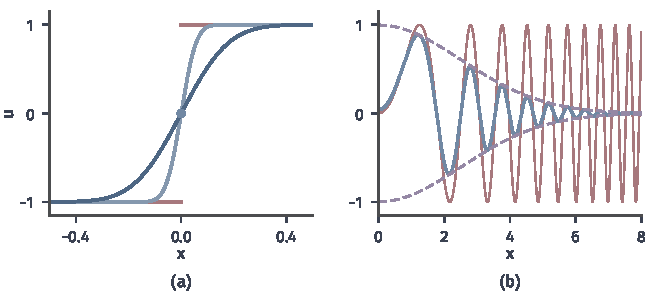
\includegraphics[width=112mm]{figures/06-differential-equations/02-partial-differential-equations/matplotlib/heat-sup-failure/figure.pdf}
  \caption{有界初值的一致恢复可能失败。(a)$u_0=\operatorname{sign}(x)$（红）与$t=0.001,0.01$的解（蓝色由浅到深），解在原点恒为零（蓝点）。(b)$u_0=\sin(x^2)$（红，细线）、$t=0.02$的解（蓝）与其包络（紫色虚线）。}
  \label{fig:heat-sup-failure}
\end{BookInlineFigure}

表~\ref{tab:heat-recovery}汇总了本节的结论。

\begin{BookInlineTable}
  \centering
  \caption{全空间热传播的初值恢复。}
  \label{tab:heat-recovery}
  \begin{tabular}{lll}
    \toprule
    初值 & 恢复方式 & 依据\\
    \midrule
    有界一致连续（含$C_0$） & 一致收敛 & 定理~\ref{thm:heat-uniform-recovery}\\
    $L^p$，$1\leq p<\infty$ & $L^p$收敛 & 定理~\ref{thm:heat-lp-recovery}\\
    满足式~\eqref{eq:heat-integrability} & 连续点处逐点收敛 & 定理~\ref{thm:heat-pointwise-recovery}\\
    一般$L^\infty$ & 一致收敛可能失败 & $\operatorname{sign}(x)$，$\sin(x^2)$\\
    \bottomrule
  \end{tabular}
\end{BookInlineTable}


\section{受迫响应}
\label{sec:heat-forced}

前面的解都由初值产生。如果棒上有持续的热源，或者端点的温度随时间改变，解又是什么？方程是线性的，答案的思路只有一条：把外部输入切成小片，每一片都当成一次自由演化的起点，再叠加起来。

\paragraph{从常微分方程到扩散}
线性常微分方程$\dot{\bm{x}}=\bm{A}\bm{x}+\bm{g}(t)$的解是
\[
 \bm{x}(t)=\mathrm{e}^{t\bm{A}}\bm{x}_0+\int_0^t\mathrm{e}^{(t-s)\bm{A}}\bm{g}(s)\,\mathrm{d}s .
\]
积分号下的读法是：时刻$s$注入的增量$\bm{g}(s)\,\mathrm{d}s$随后按齐次方程走了$t-s$的时间。

扩散的情形完全一样。时间片$[s,s+\Delta s]$内注入的热量分布大约是$f(\cdot,s)\Delta s$，它接下来自由扩散$t-s$的时间。把所有时间片的贡献加起来，令$\Delta s\to0$，得到\term{Duhamel公式}（Duhamel formula）。

\paragraph{全空间的表示}
对全空间，自由扩散由热核给出，于是
\begin{equation}
 u(\bm{x},t)=\int_{\mathbb{R}^{d}}G(\bm{x}-\bm{y},t)\,u_0(\bm{y})\,\mathrm{d}\bm{y}+\int_0^t\!\!\int_{\mathbb{R}^{d}}G(\bm{x}-\bm{y},t-s)\,f(\bm{y},s)\,\mathrm{d}\bm{y}\,\mathrm{d}s .
 \label{eq:heat-duhamel-space}
\end{equation}
图~\ref{fig:heat-duhamel-pulses}取$\lvert x\rvert<1/4$上的单位热源，持续到$t=0.5$，切成五片。较晚注入的片（深色）还很集中，较早注入的已经散开，它们的和（绿点）贴近精确的积分（蓝）。

\begin{BookInlineFigure}
  \centering
  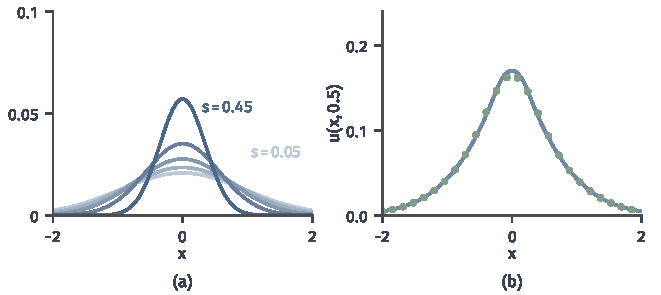
\includegraphics[width=112mm]{figures/06-differential-equations/02-partial-differential-equations/matplotlib/heat-duhamel-pulses/figure.pdf}
  \caption{热源$f=\mathbb{I}_{[-1/4,1/4]}(x)$，$0<s<0.5$，初值为零，观察时刻$t=0.5$。(a)五个时间片（$s=0.05,0.15,\ldots,0.45$，$\Delta s=0.1$）各自的响应，颜色越深注入越晚。(b)五片之和（绿点）与时间积分的精确结果（蓝）。}
  \label{fig:heat-duhamel-pulses}
\end{BookInlineFigure}

把这个想法变成定理，难点在$s\to t$时核变成奇异的。只要把时间积分靠近奇异点的一段切开，用热核收回初值的性质来处理。

\begin{theorem}[全空间的Duhamel公式]
\label{thm:heat-duhamel-space}
设$f$及其导数$\partial_tf$、$\partial_{x_i}f$、$\partial_{x_i}\partial_{x_j}f$在$\mathbb{R}^{d}\times[0,T]$上有界连续，并取$u_0=0$。则式~\eqref{eq:heat-duhamel-space}的第二项给出的$u$在$\mathbb{R}^{d}\times(0,T]$上有连续的$\partial_tu$与二阶空间偏导，并满足
\begin{equation}
 \partial_tu=\Delta u+f,\qquad \lim_{t\to0^+}\sup_{\bm{x}}\lvert u(\bm{x},t)\rvert=0 .
 \label{eq:heat-duhamel-solves}
\end{equation}
\end{theorem}

\begin{proof}
由$\int G=1$，$\lvert u(\bm{x},t)\rvert\leq t\sup\lvert f\rvert$，这给出初值条件。

为了求导，先把$\bm{y}$和$s$都换成相对量，令$\bm{y}\mapsto\bm{x}-\bm{y}$、$s\mapsto t-s$：
\[
 u(\bm{x},t)=\int_0^t\!\!\int G(\bm{y},s)\,f(\bm{x}-\bm{y},t-s)\,\mathrm{d}\bm{y}\,\mathrm{d}s .
\]
现在$\bm{x}$和$t$只出现在光滑的$f$中，可以在积分号下求导：
\[
 \Delta u=\int_0^t\!\!\int G(\bm{y},s)\,\Delta f(\bm{x}-\bm{y},t-s)\,\mathrm{d}\bm{y}\,\mathrm{d}s,
\]
\[
 \partial_tu=\int_0^t\!\!\int G(\bm{y},s)\,\partial_tf(\bm{x}-\bm{y},t-s)\,\mathrm{d}\bm{y}\,\mathrm{d}s+\int G(\bm{y},t)f(\bm{x}-\bm{y},0)\,\mathrm{d}\bm{y} .
\]
记$F(\bm{y},s)=f(\bm{x}-\bm{y},t-s)$，则$\partial_tf=-\partial_sF$，$\Delta f=\Delta_{\bm{y}}F$。相减，并把时间积分在小的$\varepsilon>0$处切开：
\[
 (\partial_t-\Delta)u=\int_\varepsilon^t\!\!\int G\,(-\partial_s-\Delta_{\bm{y}})F\,\mathrm{d}\bm{y}\,\mathrm{d}s+R_\varepsilon+\int G(\bm{y},t)F(\bm{y},t)\,\mathrm{d}\bm{y},
\]
其中$R_\varepsilon$是$[0,\varepsilon]$上的积分，由导数有界，$\lvert R_\varepsilon\rvert\leq C\varepsilon$。

第一项在$[\varepsilon,t]$上对$s$和$\bm{y}$分部积分，这里$G$光滑且快速衰减，边界只出现在$s=\varepsilon$和$s=t$：
\[
 \int_\varepsilon^t\!\!\int(\partial_sG-\Delta G)F\,\mathrm{d}\bm{y}\,\mathrm{d}s+\int G(\bm{y},\varepsilon)F(\bm{y},\varepsilon)\,\mathrm{d}\bm{y}-\int G(\bm{y},t)F(\bm{y},t)\,\mathrm{d}\bm{y} .
\]
第一个积分为零，最后一项恰好与前面的$\int G(\bm{y},t)F(\bm{y},t)\,\mathrm{d}\bm{y}$抵消。于是
\[
 (\partial_t-\Delta)u=\int G(\bm{y},\varepsilon)f(\bm{x}-\bm{y},t-\varepsilon)\,\mathrm{d}\bm{y}+R_\varepsilon .
\]
令$\varepsilon\to0^+$。$f$有界且导数有界，所以一致连续，用定理~\ref{thm:heat-uniform-recovery}同样的分段估计，右端趋于$f(\bm{x},t)$。导数的连续性由积分号下的表达式得到。
\end{proof}

这里要求$f$光滑，是因为导数都放在了$f$上。降低$f$的正则性时，经典解可能不存在，式~\eqref{eq:heat-duhamel-space}仍然可以作为一个积分定义的解，这一点在解半群一节再说。

\begin{example}[恒定点源]
\label{ex:heat-line-point-source}
实轴原点处有单位强度的恒定点源，初值为零。它不满足定理的光滑要求，但式~\eqref{eq:heat-duhamel-space}中的积分仍有意义，给出$u(x,t)=\int_0^tG(x,s)\,\mathrm{d}s$。在原点，
\[
 u(0,t)=\int_0^t\frac{\mathrm{d}s}{\sqrt{4\pi s}}=\sqrt{\frac{t}{\pi}} .
\]
$t=1$时为$0.5642$，$t=4$时为$1.1284$，无限增长。实轴上一维的点源没有稳态，因为热量散开的速度跟不上注入的速度。
\end{example}

图~\ref{fig:heat-line-point-source}对比了这一点。区间上情形不同。在$(0,1)$的中点放同样的单位点源，两端保持为零，温度有界，稳态是折线$\tfrac12\min\{x,1-x\}$，中点的值是$1/4$：吸热的端点把注入的热量带走了。

\begin{BookInlineFigure}
  \centering
  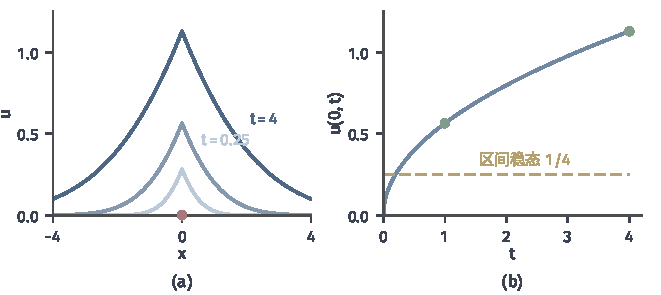
\includegraphics[width=112mm]{figures/06-differential-equations/02-partial-differential-equations/matplotlib/heat-line-point-source/figure.pdf}
  \caption{实轴上原点处的恒定单位点源（红点）。(a)$t=0.25,1,4$时的温度（蓝色由浅到深），原点处有一个折角。(b)原点温度$\sqrt{t/\pi}$（蓝）无限增长，绿点是$t=1,4$的值；黄色虚线是$(0,1)$上中点受单位点源、两端为零时的稳态值$1/4$。}
  \label{fig:heat-line-point-source}
\end{BookInlineFigure}

\paragraph{边界模式的表示}
在区间上自由演化由模式给出，同样的切片思想逐个模式进行。设$u$按$e_k$展开，系数记为$a_k(t)$，$f_k(t)=\langle f(\cdot,t),e_k\rangle$。用$e_k$检验$\partial_tu=\partial_x^2u+f$，分部积分两次，端点项因零边值而消失，每个模式得到一个独立的标量方程：
\[
 a_k'(t)=-\lambda_ka_k(t)+f_k(t) .
\]
这是一个标准的一阶线性方程，解出
\begin{equation}
 a_k(t)=\mathrm{e}^{-\lambda_kt}a_k(0)+\int_0^t\mathrm{e}^{-\lambda_k(t-s)}f_k(s)\,\mathrm{d}s .
 \label{eq:heat-duhamel-modes}
\end{equation}

把系数合起来，并定义区间上的核
\begin{equation}
 G_D(x,y,t)=\sum_{k\geq1}e_k(x)e_k(y)\mathrm{e}^{-\lambda_kt},
 \label{eq:heat-dirichlet-kernel}
\end{equation}
式~\eqref{eq:heat-duhamel-modes}就写成了与式~\eqref{eq:heat-duhamel-space}同样的形状，只是$G(x-y,t-s)$换成了$G_D(x,y,t-s)$。这个核依赖$x$和$y$两个变量，不只是它们的差，因为端点破坏了平移不变性。

当$f:[0,T]\to L^2(0,1)$连续时，由$\lvert\int_0^t\mathrm{e}^{-\lambda_k(t-s)}f_k\,\mathrm{d}s\rvert$的Cauchy--Schwarz估计，级数在$L^2$中收敛，定义了一个$L^2$值的解。若$f$、$\partial_xf$、$\partial_x^2f$在$[0,1]\times[0,T]$上连续且$f$在端点为零，分部积分两次给出$\sup_s\lvert f_k(s)\rvert\leq C/k^2$。又由时间积分的直接估计，
\[
 \lambda_k\Bigl\lvert\int_0^t\mathrm{e}^{-\lambda_k(t-s)}f_k(s)\,\mathrm{d}s\Bigr\rvert\leq\sup_s\lvert f_k(s)\rvert .
\]
于是$\sum_k\lambda_k\lvert a_k\rvert$的受迫部分可和，级数可以逐项求导，得到经典解。

\begin{example}[恒定热源趋于稳态]
\label{ex:heat-source-steady}
在$(0,1)$上取$f=1$，$u_0=0$，两端为零。系数为
\[
 f_k=\sqrt2\int_0^1\sin(k\pi x)\,\mathrm{d}x=\frac{\sqrt2\,(1-(-1)^k)}{k\pi},
\]
奇数$k$上等于$2\sqrt2/(k\pi)$，偶数$k$上为零。由式~\eqref{eq:heat-duhamel-modes}，对恒定的$f_k$积分，
\[
 a_k(t)=\frac{f_k}{\lambda_k}\bigl(1-\mathrm{e}^{-\lambda_kt}\bigr) .
\]
$t\to\infty$时$a_k\to f_k/\lambda_k$，这正是$-u''=1$、零边值的稳态解$x(1-x)/2$的系数，$-\partial_x^2$在模式坐标中就是乘以$\lambda_k$。在中点，稳态值是$1/8$。
\end{example}

这个$f$在端点不为零，上面逐项求导的充分条件不适用，但解可以直接写成稳态减去自由衰减：
\[
 u=\frac{x(1-x)}{2}-\sum_k\frac{f_k}{\lambda_k}\mathrm{e}^{-\lambda_kt}e_k .
\]
第一项是多项式，第二项属于定理~\ref{thm:heat-series}的情形，所以$t>0$时仍是经典解。

中点的值由这个级数算出，$t=0.05,0.1,0.2,0.5$时依次是
\[
 0.0463,\quad 0.0769,\quad 0.1071,\quad 0.1241 .
\]
图~\ref{fig:heat-source-steady}(b)说明每个模式按自己的速度靠近稳态，最慢的是$k=1$，高频模式几乎立刻到位。

\begin{BookInlineFigure}
  \centering
  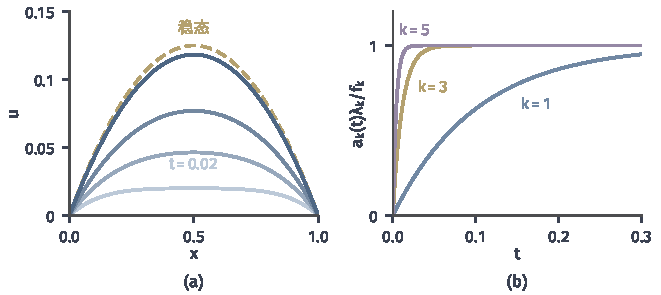
\includegraphics[width=112mm]{figures/06-differential-equations/02-partial-differential-equations/matplotlib/heat-source-steady/figure.pdf}
  \caption{恒定热源$f=1$，零边值，零初值。(a)$t=0.02,0.05,0.1,0.3$的解（蓝色由浅到深）趋于稳态$x(1-x)/2$（黄色虚线）。(b)各模式到稳态的比例$a_k(t)\lambda_k/f_k=1-\mathrm{e}^{-\lambda_kt}$，$k=1,3,5$。}
  \label{fig:heat-source-steady}
\end{BookInlineFigure}

\paragraph{非齐次边界的提升}
模式展开依赖零边值：分部积分时端点项才会消失。端点温度$u(0,t)=g_0(t)$、$u(1,t)=g_1(t)$非零时，先减去一个满足边界条件的函数，这称为\term{边界提升}（boundary lifting）。

设$g_0,g_1\in C^1[0,T]$，取线性插值
\[
 w(x,t)=(1-x)g_0(t)+xg_1(t) .
\]
令$v=u-w$。于是$v$在两端为零，而$\partial_x^2w=0$，代入原方程得到
\begin{equation}
 \partial_tv=\partial_x^2v+f-\partial_tw,\qquad v(x,0)=u_0(x)-w(x,0) .
 \label{eq:heat-lift-problem}
\end{equation}
边值变化的代价是多了一项源$-\partial_tw$，这就是要求$g_0,g_1$可微的原因。$v$现在可以用式~\eqref{eq:heat-duhamel-modes}求解。

Neumann情形要求端点斜率分别为$g_0$、$g_1$，提升不能用线性函数，因为一条直线只有一个斜率。取二次函数
\[
 w=g_0x+\frac{g_1-g_0}{2}x^2 ,
\]
这时$\partial_x^2w=g_1-g_0$不为零，$v=u-w$的源项是$f+\partial_x^2w-\partial_tw$。多维区域上可以用第~\ref{chap:elliptic-equations}章的调和函数作提升：取$\Delta w=0$、边界上$w=g$，再按上面的方式处理。

\begin{example}[一端突然加热]
\label{ex:heat-boundary-lift}
取$u_0=0$，$u(0,t)=0$，$u(1,t)=1$。提升函数是$w=x$，不随时间变化，于是$v$满足无源的热方程，初值$-x$。$x$在$e_k$上的坐标是$\sqrt2(-1)^{k+1}/(k\pi)$，所以
\[
 u(x,t)=x+\sum_{k\geq1}\frac{2(-1)^k}{k\pi}\,\mathrm{e}^{-k^2\pi^2t}\sin(k\pi x) .
\]
在中点，$t=0.05,0.1,0.2,0.5$的温度分别是
\[
 0.1138,\quad 0.2628,\quad 0.4116,\quad 0.4954 ,
\]
趋于稳态$w(1/2)=1/2$。
\end{example}

这个例子的初值和边值在$(1,0)$处矛盾，$v$的初值$-x$在$x=1$不为零，所以属于定理~\ref{thm:heat-series}的$L^2$情形，$t>0$时光滑。图~\ref{fig:heat-boundary-lift}中，(a)是$v$的衰减，(b)是加回$w$之后的$u$。

\begin{BookInlineFigure}
  \centering
  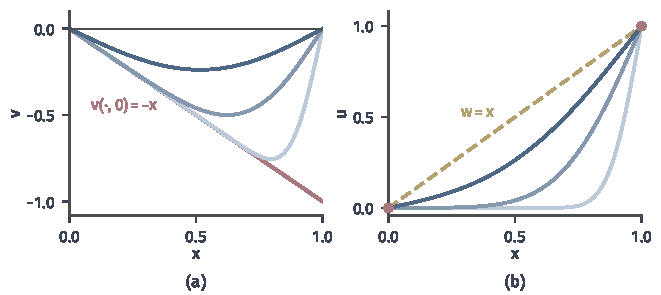
\includegraphics[width=112mm]{figures/06-differential-equations/02-partial-differential-equations/matplotlib/heat-boundary-lift/figure.pdf}
  \caption{边界提升，$u(0,t)=0$，$u(1,t)=1$，$u_0=0$，$t=0.005,0.03,0.1$（蓝色由浅到深）。(a)$v=u-w$，初值$-x$（红），两端为零。(b)$u=w+v$，黄色虚线是提升函数$w=x$，红点是边值。}
  \label{fig:heat-boundary-lift}
\end{BookInlineFigure}

\paragraph{全空间公式不能照搬}
既然有了卷积公式，能否直接把区间上的初值代进去？把三角形延拓成零，用实轴的核做卷积，图~\ref{fig:heat-wholeline-vs-interval}(a)的黄线就是结果。在$t=0.05$时它在端点的值约$0.111$，并不等于边值$0$，棒外的“真空”也被当成了可以吸收热量的材料。

对有特殊几何的区间，可以用\term{像源法}（method of images）修正。把初值奇延拓，再按周期$2$延拓，图~\ref{fig:heat-wholeline-vs-interval}(b)的红线就是这个延拓。这个函数在$x=0,1$两侧反对称，实轴上的卷积保持对称性，所以解在这些点始终为零。

\begin{BookInlineFigure}
  \centering
  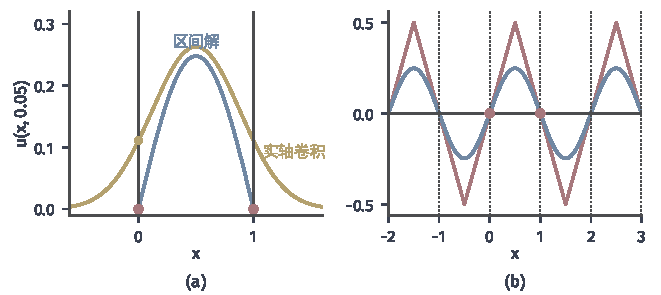
\includegraphics[width=112mm]{figures/06-differential-equations/02-partial-differential-equations/matplotlib/heat-wholeline-vs-interval/figure.pdf}
  \caption{实轴卷积与区间问题，三角形初值，$t=0.05$。(a)区间解（蓝）在端点（红点）为零；把三角形延拓为零后的实轴卷积（黄）在端点的值约$0.111$。深灰竖线是棒的端点。(b)奇延拓并按周期$2$延拓的初值（红）与实轴卷积（蓝），解在每个整数点为零。}
  \label{fig:heat-wholeline-vs-interval}
\end{BookInlineFigure}

用公式写出来，把周期延拓代入卷积，就得到另一种形式的区间核：
\begin{equation}
 G_D(x,y,t)=\sum_{n\in\mathbb{Z}}\bigl(G(x-y+2n,t)-G(x+y+2n,t)\bigr) .
 \label{eq:heat-image-kernel}
\end{equation}
它和式~\eqref{eq:heat-dirichlet-kernel}是同一个函数的两种写法，因为两者给出同一个问题的解，而解是唯一的，唯一性在第~\ref{sec:heat-properties}节证明。像源的写法在$t$小时收敛极快，只需$n=0$的项；模式的写法在$t$大时收敛极快，只需前几项。对图中的例子数值计算$u(1/2,0.05)$，两种写法都得到$0.24796$。一般区域没有这种反射结构，边界的作用需要由模式或其他方法处理。


\section{解的性质}
\label{sec:heat-properties}

上面几节的解都有公式，公式只存在于少数几何形状上。一般区域、一般数据时能断定什么？下面研究四个量：总热量、最高最低温度、平方积分、光滑程度。每个量的变化规律都来自对方程本身的一次计算，不需要解的表达式，并且在估计中明确写出需要什么边界和源项条件。

\subsection{质量变化}
\label{sec:heat-mass}

棒里的总热量会怎样变？这是守恒律的积分形式，它的结论最直接。记$M(t)=\int_\Omega u(\bm{x},t)\,\mathrm{d}\bm{x}$。

\begin{theorem}[质量平衡]
\label{thm:heat-mass-balance}
设$\Omega$是有界开集，边界分段$C^1$，$u$在$\overline\Omega\times(0,T]$上有连续的$\partial_tu$和二阶空间偏导，满足$\partial_tu=\Delta u+f$，$f$连续。则对$0<t\leq T$，
\begin{equation}
 M'(t)=\int_\Omega f\,\mathrm{d}\bm{x}+\int_{\partial\Omega}\partial_{\bm{n}}u\,\mathrm{d}S .
 \label{eq:heat-mass-balance}
\end{equation}
\end{theorem}

\begin{proof}
被积函数连续，可以在积分号下对$t$求导：$M'(t)=\int_\Omega(\Delta u+f)\,\mathrm{d}\bm{x}$。由散度定理，$\Delta u=\nabla\cdot\nabla u$的体积分等于$\partial_{\bm{n}}u$的边界积分。这就是式~\eqref{eq:heat-mass-balance}。
\end{proof}

右端两项是两个不同的来源：内部源项的贡献和穿过边界的净通量。于是可以分情形读。

无源且零Neumann条件时，右端为零，总质量守恒。无源且零Dirichlet条件时，边界项一般不为零。设$u\geq0$，边界上$u=0$是最小值，温度沿外法向下降，$\partial_{\bm{n}}u\leq0$，所以$M'\leq0$，这种吸收边界让质量流失。

全空间没有边界，但需要无穷远处的衰减代替它。最直接的条件是$u_0\in L^1(\mathbb{R}^{d})$，这时由Fubini定理和$\int G=1$，
\[
 \int_{\mathbb{R}^{d}}u(\bm{x},t)\,\mathrm{d}\bm{x}=\int_{\mathbb{R}^{d}}u_0(\bm{y})\int_{\mathbb{R}^{d}}G(\bm{x}-\bm{y},t)\,\mathrm{d}\bm{x}\,\mathrm{d}\bm{y}=\int_{\mathbb{R}^{d}}u_0(\bm{y})\,\mathrm{d}\bm{y} .
\]
这里不需要任何关于导数在无穷远的假设。如果想用式~\eqref{eq:heat-mass-balance}在大球上取极限，就要证明大球面上的通量趋于零，这正是“适当衰减”的含义。

回到三角形。由式~\eqref{eq:heat-sine-solution}逐项积分，Dirichlet情形的质量是
\[
 M(t)=\sum_{k\text{ 奇}}\frac{8\sin(k\pi/2)}{k^3\pi^3}\,\mathrm{e}^{-k^2\pi^2t} .
\]
$t=0$时求和得$1/4$，$t=0.02,0.05,0.1,0.2$时依次约为
\[
 0.2102,\quad 0.1574,\quad 0.0962,\quad 0.0358 .
\]
Neumann情形$M$恒为$1/4$。对称性使两端的流出相同，式~\eqref{eq:heat-mass-balance}给出$M'=-2\partial_xu(0,t)$，$t=0.1$时左端斜率约为$0.4745$，流出率约为$0.949$，图~\ref{fig:heat-mass-balance}(b)用$M$的差商核对了这个等式。

有源时两项相互竞争。图~\ref{fig:heat-mass-balance}(c)取$f=1$，$u_0=0$。Dirichlet情形下，随着温度升高，边界流出变大，最终内部注入速率$1$被两端流出抵消，每端的斜率大小是$1/2$，质量趋于稳态的积分$\int_0^1x(1-x)/2\,\mathrm{d}x=1/12$。Neumann情形没有出口，$M(t)=t$无限增长，没有稳态，这对应着椭圆Neumann问题的相容条件$\int f=0$不成立。

\begin{BookInlineFigure}
  \centering
  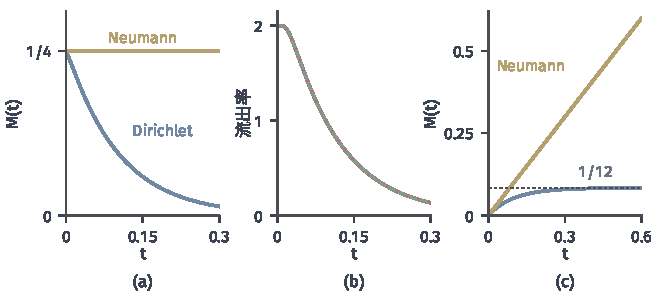
\includegraphics[width=112mm]{figures/06-differential-equations/02-partial-differential-equations/matplotlib/heat-mass-balance/figure.pdf}
  \caption{总热量的变化。(a)三角形初值、无源：Dirichlet（蓝）流失，Neumann（黄）不变。(b)Dirichlet情形的边界流出率$2\partial_xu(0,t)$（红）与$-M'(t)$的差商（绿色虚线），两者重合。(c)$f=1$、$u_0=0$：Dirichlet（蓝）趋于$1/12$，Neumann（黄）线性增长。}
  \label{fig:heat-mass-balance}
\end{BookInlineFigure}

\subsection{最大值原理}
\label{sec:heat-maximum}

没有热源时，棒内能不能出现比开始时和端点都热的点？物理上不能，热量只往低处流。数学上的结论需要指明温度的最大值可能出现在哪些地方，这就要看时空区域的边界中哪一部分真正影响解。

\paragraph{抛物边界}
记$\Omega_T=\Omega\times(0,T]$。称底面与侧面的并
\[
 \Gamma_T=(\overline\Omega\times\{0\})\cup(\partial\Omega\times[0,T])
\]
为\term{抛物边界}（parabolic boundary），它就是给定数据的那部分，图~\ref{fig:heat-parabolic-boundary}。顶面$t=T$不在其中，因为信息只从过去流向未来，那里的值由方程决定。

\begin{BookInlineFigure}
  \centering
  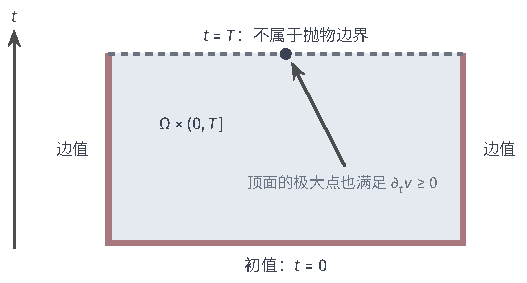
\includegraphics[width=90mm]{figures/06-differential-equations/02-partial-differential-equations/tikz/heat-parabolic-boundary/figure.pdf}
  \caption{时空矩形$\Omega\times(0,T]$的抛物边界（红色粗线）由底面和两条侧边组成，顶面（虚线）不属于它。顶面上若有极大点（黑点），那里的时间导数只能从过去一侧计算，符号仍然与方程矛盾，这正是定理的证明要点。}
  \label{fig:heat-parabolic-boundary}
\end{BookInlineFigure}

\begin{theorem}[弱最大值原理]
\label{thm:heat-weak-max}
设$\Omega$是有界开集，$u\in C(\overline\Omega\times[0,T])$，在$\Omega_T$上$\partial_tu$和二阶空间偏导连续，且$\partial_tu-\Delta u\leq0$。则
\begin{equation}
 \max_{\overline\Omega\times[0,T]}u=\max_{\Gamma_T}u .
 \label{eq:heat-weak-max}
\end{equation}
\end{theorem}

\begin{proof}
如果严格不等式$\partial_tv-\Delta v<0$成立，论证很短，所以先制造严格性。任取$\varepsilon>0$，令$v=u-\varepsilon t$，则
\[
 \partial_tv-\Delta v=\partial_tu-\Delta u-\varepsilon<0 .
\]
$v$在紧集上连续，在某点$(\bm{x}_0,t_0)$取得最大值。假设这一点不在$\Gamma_T$上，即$\bm{x}_0\in\Omega$，$0<t_0\leq T$。

固定$t_0$，$\bm{x}_0$是$v(\cdot,t_0)$的内部极大点，Hessian半负定，于是$\Delta v(\bm{x}_0,t_0)\leq0$。固定$\bm{x}_0$看时间：若$t_0<T$，一阶条件给出$\partial_tv=0$；若$t_0=T$，$v(\bm{x}_0,t)\leq v(\bm{x}_0,T)$对$t<T$成立，左导数给出$\partial_tv\geq0$。无论哪种情形，
\[
 \partial_tv-\Delta v\geq0,
\]
与严格不等式矛盾。所以$v$的最大值在$\Gamma_T$上取到。由$0\leq\varepsilon t\leq\varepsilon T$，
\[
 \max u\leq\max v+\varepsilon T=\max_{\Gamma_T}v+\varepsilon T\leq\max_{\Gamma_T}u+\varepsilon T .
\]
令$\varepsilon\to0$，得$\max u\leq\max_{\Gamma_T}u$。反方向的不等式成立是因为$\Gamma_T$是整个闭集的子集。
\end{proof}

条件$\partial_tu-\Delta u\leq0$的含义是内部不产生热量，可以吸热。对$-u$用定理，就得到$\partial_tu-\Delta u\geq0$时最小值在$\Gamma_T$上取到。图~\ref{fig:heat-max-envelope}中初值是$\sin(\pi x)+\sin(5\pi x)$，负的小凹陷很快被填平，最大值单调下降，最小值从$-0.198$上升到$0$，都不越出初值和边界值的范围。

\begin{BookInlineFigure}
  \centering
  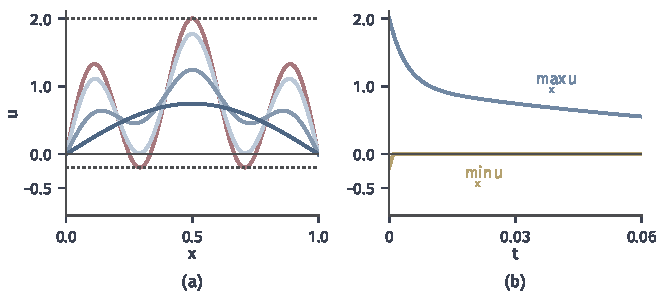
\includegraphics[width=112mm]{figures/06-differential-equations/02-partial-differential-equations/matplotlib/heat-max-envelope/figure.pdf}
  \caption{最大值原理的例子，$u_0=\sin(\pi x)+\sin(5\pi x)$（红），两端为零。(a)$t=0.001,0.005,0.03$的解（蓝色由浅到深），两条点线是初值的最大值$2$和最小值$-0.198$。(b)$\max_xu$（蓝）单调下降，$\min_xu$（黄）单调上升到$0$。}
  \label{fig:heat-max-envelope}
\end{BookInlineFigure}

这里要注意定理比较的是抛物边界上的值。零Neumann条件下侧面的值未知，定理不能直接说最大值在底面。一维时可以用偶延拓把隔热端点变成对称的内部点，再用全空间的结论，就知道隔热棒的最高温也不超过初值的最高温。一般区域上的同一结论需要边界点处法向导数的符号引理，篇幅较长，读者可查阅抛物方程的教材。

\paragraph{比较、唯一与连续依赖}
线性方程的两个解相减仍是解，把弱最大值原理用在差上，立刻得到几条结论。

\begin{theorem}[比较原理与唯一性]
\label{thm:heat-comparison}
设$\Omega$是有界开集，$u_1,u_2$满足定理~\ref{thm:heat-weak-max}的正则性，记$Lu=\partial_tu-\Delta u$。
\begin{enumerate}
 \item 若在$\Omega_T$上$Lu_1\leq Lu_2$，在$\Gamma_T$上$u_1\leq u_2$，则处处$u_1\leq u_2$。
 \item 若$Lu_i=f_i$，记$F=\sup_{\Omega_T}\lvert f_1-f_2\rvert$，则
 \begin{equation}
  \max\lvert u_1-u_2\rvert\leq\max_{\Gamma_T}\lvert u_1-u_2\rvert+TF .
  \label{eq:heat-max-stability}
 \end{equation}
 \item 特别地，Dirichlet初边值问题的经典解至多一个。
\end{enumerate}
\end{theorem}

\begin{proof}
(1)对$u_1-u_2$用定理~\ref{thm:heat-weak-max}。

(2)令$w=u_1-u_2-Ft$，则$\partial_tw-\Delta w=f_1-f_2-F\leq0$。由定理~\ref{thm:heat-weak-max}和$-Ft\leq0$，
\[
 \max(u_1-u_2)\leq\max w+FT\leq\max_{\Gamma_T}(u_1-u_2)+FT .
\]
交换$u_1$与$u_2$得到另一方向。

(3)在式~\eqref{eq:heat-max-stability}中令数据相同，右端为零。
\end{proof}

比较原理使我们能用简单的函数夹住解。例如例~\ref{ex:heat-source-steady}中$f=1$、$u_0=0$：与$w=t$比较，$\partial_tw-\partial_x^2w=1=f$，抛物边界上$u\leq w$，于是$u\leq t$；再与稳态$x(1-x)/2$比较，又有$u\leq x(1-x)/2$。前面算出$t=0.05$时中点值是$0.0463$，确实不超过$0.05$，也不超过$0.125$。

\paragraph{全空间与增长限制}
有界区域的证明用到了最大值存在，这在全空间不再自动成立，结论本身也可能失败。存在一族Tikhonov解，由
\[
 u(x,t)=\sum_{m\geq0}\frac{x^{2m}}{(2m)!}\,\phi^{(m)}(t),\qquad \phi(t)=\mathrm{e}^{-t^{-\alpha}}\ (\alpha>1,\ t>0),\quad \phi(0)=0
\]
给出，它在实轴上满足热方程，初值为零，却不恒为零。这个例子的收敛性验证较长，读者可查阅偏微分方程的教材。它的增长比$\mathrm{e}^{ax^2}$还快，这是无穷远处传进来的“幽灵热量”。下面的定理说明，只要禁止这样的增长，最大值原理就恢复了。

\begin{theorem}[全空间的最大值原理]
\label{thm:heat-whole-max}
设$u\in C(\mathbb{R}^{d}\times[0,T])$，在$\mathbb{R}^{d}\times(0,T]$上$\partial_tu$和二阶空间偏导连续，$\partial_tu-\Delta u\leq0$，并存在常数$A,a>0$，使
\begin{equation}
 u(\bm{x},t)\leq A\,\mathrm{e}^{a\lvert\bm{x}\rvert^2},\qquad \bm{x}\in\mathbb{R}^{d},\ 0\leq t\leq T .
 \label{eq:heat-growth}
\end{equation}
若$M_0=\sup u_0<\infty$，则$u\leq M_0$处处成立。特别地，若两个解的绝对值都满足式~\eqref{eq:heat-growth}这样的界，初值相同则解相同。
\end{theorem}

\begin{proof}
先设$4aT<1$，取$\varepsilon>0$使$4a(T+\varepsilon)<1$，并记$a+\gamma=1/(4(T+\varepsilon))$，$\gamma>0$。固定$\bm{y}\in\mathbb{R}^{d}$、$\mu>0$，引入一个向无穷增长、满足方程的比较函数。记$\rho=T+\varepsilon-t>0$，令
\[
 w(\bm{x},t)=\rho^{-d/2}\exp\Bigl(\frac{\lvert\bm{x}-\bm{y}\rvert^2}{4\rho}\Bigr) .
\]
直接求导，$\partial_tw$和$\Delta w$都等于$\bigl(\tfrac{d}{2\rho}+\tfrac{\lvert\bm{x}-\bm{y}\rvert^2}{4\rho^2}\bigr)w$，所以$\partial_tw=\Delta w$。令$v=u-\mu w$，则$\partial_tv-\Delta v\leq0$。

在球$B_r(\bm{y})$上用定理~\ref{thm:heat-weak-max}，只需看抛物边界。底面上$w>0$，所以$v\leq u_0\leq M_0$。侧面$\lvert\bm{x}-\bm{y}\rvert=r$上，用式~\eqref{eq:heat-growth}和$\rho\leq T+\varepsilon$，
\[
 v\leq A\,\mathrm{e}^{a(\lvert\bm{y}\rvert+r)^2}-\mu\,(T+\varepsilon)^{-d/2}\,\mathrm{e}^{(a+\gamma)r^2} .
\]
$r\to\infty$时第二项的指数系数$a+\gamma$大于第一项的$a$，右端趋于$-\infty$，于是$r$足够大时$v\leq M_0$。

由定理~\ref{thm:heat-weak-max}，$v\leq M_0$在球内成立。在球心取值，得$u(\bm{y},t)\leq M_0+\mu\,w(\bm{y},t)$。$w(\bm{y},t)=\rho^{-d/2}$有界，令$\mu\to0$，得$u(\bm{y},t)\leq M_0$。

一般的$T$，把$[0,T]$分成长度不超过$1/(8a)$的小段，逐段应用上面的结论，每一段的初值都不超过$M_0$。唯一性：两个解的差及其相反数都满足定理的条件，初值的上确界为零，差恒为零。
\end{proof}

增长条件的常数$a$可以任意大，$T$也可以任意大，不过$\mathrm{e}^{a\lvert\bm{x}\rvert^2}$这样的阶不能放宽，Tikhonov解正好越过这条线。这与定理~\ref{thm:heat-convolution-smooth}的积分条件相呼应：两者都以Gauss函数的增长为界。

\subsection{能量估计}
\label{sec:heat-energy}

最大值原理控制的是最坏的一点，并且依赖边界上的符号。另一种度量是平方积分，它在两种齐次边界下都表现得很好，而且自然地连接到弱解。记$E(t)=\tfrac12\lVert u(\cdot,t)\rVert_2^2$。

\begin{theorem}[能量估计]
\label{thm:heat-energy}
设$\Omega$是有界开集，边界分段$C^1$，$u\in C(\overline\Omega\times[0,T])$，在$\overline\Omega\times(0,T]$上$\partial_tu$和二阶空间偏导连续，满足$\partial_tu=\Delta u+f$（$f$连续）及零Dirichlet条件或零Neumann条件。则对$0<t\leq T$，
\begin{equation}
 \frac12\frac{\mathrm{d}}{\mathrm{d}t}\lVert u\rVert_2^2+\lVert\nabla u\rVert_2^2=\langle f,u\rangle .
 \label{eq:heat-energy-identity}
\end{equation}
无源时，对$0<t\leq T$还有
\begin{equation}
 \frac12\lVert u(\cdot,t)\rVert_2^2+\int_0^t\lVert\nabla u\rVert_2^2\,\mathrm{d}s=\frac12\lVert u_0\rVert_2^2 .
 \label{eq:heat-energy-integrated}
\end{equation}
一般地，零Neumann时取$\mu=0$，零Dirichlet时取$\mu=1/C_P^2$，其中$C_P$是Poincaré常数，则
\begin{equation}
 \lVert u(\cdot,t)\rVert_2\leq\mathrm{e}^{-\mu t}\lVert u_0\rVert_2+\int_0^t\mathrm{e}^{-\mu(t-s)}\lVert f(\cdot,s)\rVert_2\,\mathrm{d}s .
 \label{eq:heat-energy-bound}
\end{equation}
\end{theorem}

\begin{proof}
用$u$乘方程并在$\Omega$上积分。由Green公式，
\[
 \int_\Omega u\,\Delta u\,\mathrm{d}\bm{x}=-\lVert\nabla u\rVert_2^2+\int_{\partial\Omega}u\,\partial_{\bm{n}}u\,\mathrm{d}S .
\]
两种边界条件都使边界积分为零，一种因为$u=0$，另一种因为$\partial_{\bm{n}}u=0$。这就是式~\eqref{eq:heat-energy-identity}。

无源时把式~\eqref{eq:heat-energy-identity}在$[\varepsilon,t]$上积分。令$\varepsilon\to0^+$，$u$在闭集上连续，$E(\varepsilon)\to E(0)$；由单调收敛定理，梯度项收敛，这样得到式~\eqref{eq:heat-energy-integrated}。

为了得到式~\eqref{eq:heat-energy-bound}，想对$\lVert u\rVert_2$求导，但它在零点不可微，所以任取$\varepsilon>0$，令$y=(\lVert u\rVert_2^2+\varepsilon)^{1/2}$。由式~\eqref{eq:heat-energy-identity}和Cauchy--Schwarz不等式，以及$\lVert\nabla u\rVert_2^2\geq\mu\lVert u\rVert_2^2$（Neumann时$\mu=0$，这个不等式平凡；Dirichlet时是Poincaré不等式），
\[
 y\,y'\leq-\mu\lVert u\rVert_2^2+\lVert f\rVert_2\lVert u\rVert_2 .
\]
两边除以$y>0$，用$\lVert u\rVert_2\leq y$和$\lVert u\rVert_2^2/y\geq y-\sqrt\varepsilon$，
\[
 y'\leq-\mu y+\mu\sqrt\varepsilon+\lVert f\rVert_2 .
\]
乘积分因子$\mathrm{e}^{\mu t}$积分，令$\varepsilon\to0$，就得到式~\eqref{eq:heat-energy-bound}。
\end{proof}

式~\eqref{eq:heat-energy-integrated}有两层含义。第一，能量单调下降，下降的量正是梯度的平方积分，起伏越大，耗散越快。第二，即使初值只属于$L^2$，梯度在时间上的平方积分也不超过$\tfrac12\lVert u_0\rVert_2^2$，这是后面平滑效应的积分形式。

在$(0,1)$上零Dirichlet时最优的$C_P=1/\pi$，式~\eqref{eq:heat-energy-bound}无源时就是式~\eqref{eq:heat-series-decay}，能量方法不用模式得到了同样的衰减率。

\paragraph{用于比较两组数据}
方程线性，两个解的差满足同类问题，把式~\eqref{eq:heat-energy-bound}用在差上就是对数据的连续依赖：
\begin{equation}
 \lVert u_1(t)-u_2(t)\rVert_2\leq\mathrm{e}^{-\mu t}\lVert u_{1,0}-u_{2,0}\rVert_2+\int_0^t\mathrm{e}^{-\mu(t-s)}\lVert f_1-f_2\rVert_2\,\mathrm{d}s .
 \label{eq:heat-energy-stability}
\end{equation}
数据相同则差为零，所以这也给出唯一性，并且包括零Neumann问题，这是弱最大值原理没有直接给出的。

\begin{example}[两组初值的差]
\label{ex:heat-energy-difference}
在$(0,1)$上取零边值，$u_{1,0}$为三角形，第二组初值是
\[
 u_{2,0}=u_{1,0}+\tfrac{1}{10}(\sin\pi x+\sin3\pi x) .
\]
差的初值范数是$\tfrac{1}{10}\sqrt{1/2+1/2}=0.1$，而差本身是
\[
 u_2-u_1=\tfrac{1}{10}\bigl(\mathrm{e}^{-\pi^2t}\sin\pi x+\mathrm{e}^{-9\pi^2t}\sin3\pi x\bigr) .
\]
由正交性，其范数是$\tfrac{1}{10}(\tfrac12\mathrm{e}^{-2\pi^2t}+\tfrac12\mathrm{e}^{-18\pi^2t})^{1/2}$，不超过上界$0.1\,\mathrm{e}^{-\pi^2t}$。
\end{example}

\paragraph{能量衰减与质量守恒}
能量和质量是两个不同的量，隔热棒把这一点显示得最清楚：总质量不变，能量仍在减少。由Cauchy--Schwarz不等式，$M^2\leq\lvert\Omega\rvert\,\lVert u\rVert_2^2$，等号当且仅当$u$为常数。所以在质量固定时，均匀分布的能量最小，扩散正是把温度推向这个最小能量的状态。

三角形的初始能量是$\tfrac12\int_0^1u_0^2\,\mathrm{d}x=1/24$。在隔热棒中，最终温度是$1/4$，最终能量是$\tfrac12(1/4)^2=1/32$。两者相差的$1/96$由式~\eqref{eq:heat-energy-integrated}全部以梯度平方的时间积分耗散掉。接冰水时，能量和质量都趋于零，图~\ref{fig:heat-energy-mass}(a)。

\begin{BookInlineFigure}
  \centering
  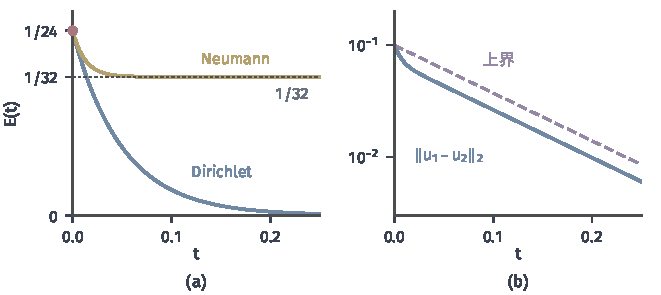
\includegraphics[width=112mm]{figures/06-differential-equations/02-partial-differential-equations/matplotlib/heat-energy-mass/figure.pdf}
  \caption{能量。(a)三角形初值（初始能量$1/24$，红点）的$E(t)$：Neumann（黄）下降到$1/32$后停止，Dirichlet（蓝）趋于$0$。(b)例~\ref{ex:heat-energy-difference}的差的$L^2$范数（蓝）与上界$0.1\,\mathrm{e}^{-\pi^2t}$（紫色虚线），纵轴为对数。}
  \label{fig:heat-energy-mass}
\end{BookInlineFigure}

上面的定理对经典解陈述。解也可以只在弱形式下成立：它在时间上平方可积地取值于$H^1_0(\Omega)$，对几乎每个$t$和每个$v\in H^1_0(\Omega)$有
\[
 \frac{\mathrm{d}}{\mathrm{d}t}\langle u,v\rangle+a(u,v)=\langle f,v\rangle ,
\]
其中$a(u,v)=\int_\Omega\nabla u\cdot\nabla v$，同样的能量等式仍然成立，取$v=u$的合法性需要取值于函数空间的时间导数理论，证明较长，读者可查阅抛物方程的教材。

表~\ref{tab:heat-three-measures}把三个度量放在一起。

\begin{BookInlineTable}
  \centering
  \caption{无源热方程的三种度量。}
  \label{tab:heat-three-measures}
  \begin{tabular}{llll}
    \toprule
    量 & 零Dirichlet & 零Neumann & 控制方式\\
    \midrule
    总质量 & 流失 & 守恒 & 边界通量\\
    最大值 & 不超过数据 & 不超过初值 & 符号结构\\
    能量 & 趋于$0$ & 趋于均匀态能量 & 梯度耗散\\
    \bottomrule
  \end{tabular}
\end{BookInlineTable}

\subsection{正时间平滑}
\label{sec:heat-smoothing}

定理~\ref{thm:heat-series}和定理~\ref{thm:heat-convolution-smooth}都说，$t>0$时解立即变成无穷光滑。这种\term{平滑效应}（smoothing effect）有多强？导数能大到什么程度？

\paragraph{全空间：把导数放到核上}
卷积的导数可以放在核上：$\partial^\alpha_{\bm{x}}u=(\partial^\alpha G)*u_0$。初值无需可导，所有的导数都由光滑的核承担，代价只是核的导数的大小。

\begin{theorem}[全空间的平滑估计]
\label{thm:heat-smoothing}
设$1\leq p\leq\infty$，$u_0\in L^p(\mathbb{R}^{d})$，$\alpha$是多重指标。则存在只依赖$\alpha$和$d$的常数$C_\alpha$，使对$t>0$，
\begin{equation}
 \lVert\partial^\alpha_{\bm{x}}u(\cdot,t)\rVert_p\leq C_\alpha\,t^{-\lvert\alpha\rvert/2}\,\lVert u_0\rVert_p .
 \label{eq:heat-smoothing}
\end{equation}
\end{theorem}

\begin{proof}
$L^p$函数满足式~\eqref{eq:heat-integrability}：由Hölder不等式，Gauss函数属于$L^{p'}$。于是定理~\ref{thm:heat-convolution-smooth}允许在积分号下求导。用定理~\ref{thm:heat-lp-recovery}证明中的Minkowski不等式，
\[
 \lVert\partial^\alpha u(\cdot,t)\rVert_p\leq\lVert\partial^\alpha G(\cdot,t)\rVert_1\,\lVert u_0\rVert_p .
\]
由尺度关系~\eqref{eq:heat-kernel-scaling}求导，
\[
 \partial^\alpha G(\bm{x},t)=t^{-(d+\lvert\alpha\rvert)/2}(\partial^\alpha G)(\bm{x}/\sqrt{t},1) .
\]
积分时代换$\bm{x}=\sqrt{t}\,\bm{z}$，因子$t^{d/2}$抵消，于是
\[
 \lVert\partial^\alpha G(\cdot,t)\rVert_1=t^{-\lvert\alpha\rvert/2}\lVert\partial^\alpha G(\cdot,1)\rVert_1 .
\]
把最后这个有限的$L^1$范数取作$C_\alpha$。
\end{proof}

一维$\alpha=1$时常数可以算出来。$G(\cdot,t)$是单峰函数，它的导数的$L^1$范数等于全变差，是峰值的两倍：
\[
 \lVert\partial_xG(\cdot,t)\rVert_1=2G(0,t)=\frac{1}{\sqrt{\pi t}} .
\]
于是
\[
 \lVert\partial_xu(\cdot,t)\rVert_\infty\leq\frac{\lVert u_0\rVert_\infty}{\sqrt{\pi t}} .
\]
这个常数不能再小：$u_0=\operatorname{sign}(x)$时$u=\operatorname{erf}(x/(2\sqrt{t}))$，在原点的斜率恰好是$1/\sqrt{\pi t}$，等号成立。

同样的办法还能把可积性换成有界性。卷积不超过核的上确界乘以$\lVert u_0\rVert_1$，于是
\[
 \lVert u(\cdot,t)\rVert_\infty\leq(4\pi t)^{-d/2}\lVert u_0\rVert_1 .
\]
这说明一点上的尖峰无法存留，只要总量有限，高度就被核的峰值控制。

\paragraph{区间：谱系数的压制}
有界区间上同样的结论由系数得到。对式~\eqref{eq:heat-sine-solution}，$\partial_x^mu$的系数比$u$多一个因子$(k\pi)^m$，而$\sqrt2\sin k\pi x$、$\sqrt2\cos k\pi x$都是标准正交系，所以
\[
 \lVert\partial_x^mu(\cdot,t)\rVert_2^2=\sum_k\lambda_k^m\,\mathrm{e}^{-2\lambda_kt}c_k^2\leq\Bigl(\sup_{\lambda>0}\lambda^m\mathrm{e}^{-2\lambda t}\Bigr)\sum_kc_k^2 .
\]
函数$\lambda^m\mathrm{e}^{-2\lambda t}$在$\lambda=m/(2t)$处取最大值，代入得到
\begin{equation}
 \lVert\partial_x^mu(\cdot,t)\rVert_2\leq\Bigl(\frac{m}{2\mathrm{e}\,t}\Bigr)^{m/2}\lVert u_0\rVert_2,\qquad t>0 .
 \label{eq:heat-spectral-smoothing}
\end{equation}
这和式~\eqref{eq:heat-smoothing}的$t^{-m/2}$一致。指数因子不管多小的$t$，都压得住任何多项式因子，这就是无穷光滑的来源；只是$t$越小，压制所需的频率越高，界就越大。

\paragraph{估计变差与初值的光滑性}
式~\eqref{eq:heat-smoothing}在$t\to0^+$时趋于无穷，这不说明解在变坏，而是说明界要为最粗糙的初值留有余地。初值的导数已经有界时，估计不必如此。

导数和卷积可交换：若$u_0$有界且一阶导数有界，则$\partial_xu=G*\partial_xu_0$，于是
\[
 \lVert\partial_xu(\cdot,t)\rVert_\infty\leq\lVert\partial_xu_0\rVert_\infty ,
\]
$t\to0^+$时没有奇性。解保持初值原有的光滑程度，只对超出这个程度的导数付出$t^{-1/2}$的代价。

图~\ref{fig:heat-smoothing-rates}用两个初值把这两件事分开。跳跃$\operatorname{sign}(x)$的一阶导数的界是$1/\sqrt{\pi t}$。折线$-\lvert x\rvert$的解满足$\partial_xu=-\operatorname{erf}(x/(2\sqrt{t}))$，一阶导数的界恒为$1$，二阶导数$\partial_x^2u=-2G(x,t)$的界是$1/\sqrt{\pi t}$：多出来的一阶导数才要付代价。跳跃的二阶导数代价是$t^{-1}$，正好多一个$t^{-1/2}$。

\begin{BookInlineFigure}
  \centering
  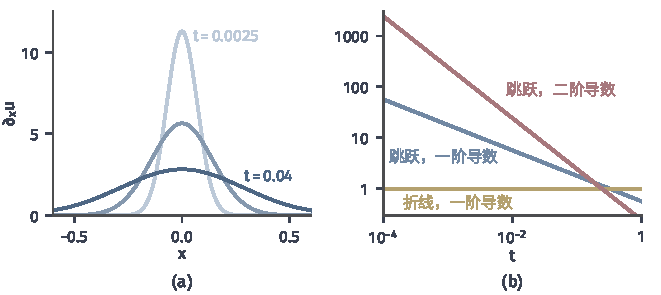
\includegraphics[width=112mm]{figures/06-differential-equations/02-partial-differential-equations/matplotlib/heat-smoothing-rates/figure.pdf}
  \caption{平滑的代价。(a)跳跃$\operatorname{sign}(x)$的解的斜率$2G(x,t)$，$t=0.0025,0.01,0.04$（蓝色由浅到深）。(b)精确的上确界，双对数坐标：跳跃的$\lVert\partial_xu\rVert_\infty=1/\sqrt{\pi t}$（蓝），跳跃的$\lVert\partial_x^2u\rVert_\infty\propto t^{-1}$（红），折线$-\lvert x\rvert$的$\lVert\partial_xu\rVert_\infty=1$（黄）。}
  \label{fig:heat-smoothing-rates}
\end{BookInlineFigure}


\section{解半群}
\label{sec:heat-semigroup}

无源时，时刻$t$的解由初值完全决定，这是一个映射。在矩阵情形，它就是$\mathrm{e}^{t\bm{A}}$，走两段时间等于把两个指数相乘。热方程的解映射是否也构成这样的结构？它的“$\bm{A}$”是什么？这需要先确定函数空间。

\paragraph{解算子与时间拼接}
把初值$u_0$映到时刻$t$的解，记为$S(t)u_0$。全空间上$S(t)u_0=G(\cdot,t)*u_0$，区间上$S(t)$把坐标$c_k$乘以$\mathrm{e}^{-\lambda_kt}$。在区间上，时间拼接就是指数相加：
\[
 \mathrm{e}^{-\lambda_k(t+s)}=\mathrm{e}^{-\lambda_kt}\,\mathrm{e}^{-\lambda_ks} .
\]

全空间上，$S(t+s)=S(t)S(s)$等价于热核的卷积恒等式
\begin{equation}
 G(\cdot,t)*G(\cdot,s)=G(\cdot,t+s),\qquad t,s>0 .
 \label{eq:heat-kernel-semigroup}
\end{equation}
证明最快的办法是取Fourier变换：左边的变换是$\mathrm{e}^{-4\pi^2\lvert\bm{\xi}\rvert^2t}\mathrm{e}^{-4\pi^2\lvert\bm{\xi}\rvert^2s}$，右边的变换是$\mathrm{e}^{-4\pi^2\lvert\bm{\xi}\rvert^2(t+s)}$，两者相等，而两边都是$L^1$函数，$L^1$上Fourier变换是单射。这个恒等式也可以从方差读出：两个独立的Gauss扰动相加，方差相加，$2t+2s=2(t+s)$。

有了式~\eqref{eq:heat-kernel-semigroup}，由Fubini定理得到$S(t)S(s)u_0=S(t+s)u_0$。图~\ref{fig:heat-semigroup-composition}用数值卷积核对了这一点：分两步走与一步走到同样的终点，差别是离散误差。这就是从时刻$s$的状态重新开始，后续演化不需要知道更早的历史。

\begin{BookInlineFigure}
  \centering
  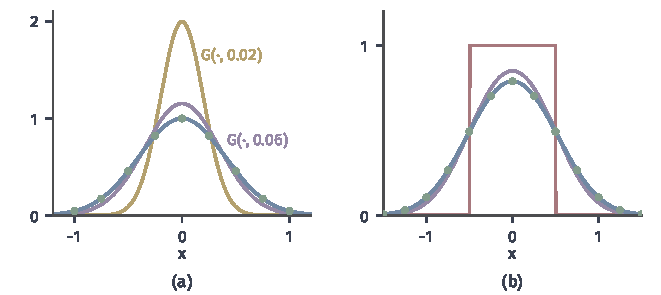
\includegraphics[width=112mm]{figures/06-differential-equations/02-partial-differential-equations/matplotlib/heat-semigroup-composition/figure.pdf}
  \caption{时间拼接。(a)$G(\cdot,0.02)$（黄）与$G(\cdot,0.06)$（紫）的数值卷积（绿点）落在$G(\cdot,0.08)$（蓝）上。(b)方框（红）先走$0.06$（紫）再走$0.02$（绿点），与一步走$0.08$的解（蓝）一致。}
  \label{fig:heat-semigroup-composition}
\end{BookInlineFigure}

\paragraph{强连续半群}
把这些性质抽象出来。注意其中只有$t\geq0$，反向一般不存在，这是“半”字的含义。

\begin{definition}[强连续半群]
\label{def:heat-c0-semigroup}
设$X$是Banach空间，$\{S(t)\}_{t\geq0}$是$X$上的有界线性算子族。若
\begin{equation}
 S(0)=I,\qquad S(t+s)=S(t)S(s),\qquad \lim_{t\to0^+}\lVert S(t)x-x\rVert_X=0
 \label{eq:heat-c0-semigroup}
\end{equation}
对所有$t,s\geq0$和$x\in X$成立，则称它是\term{强连续半群}（strongly continuous semigroup）。若还有$\lVert S(t)\rVert\leq1$，称为\term{压缩半群}（contraction semigroup）。把$u_0$映到解的这样一族算子称为\term{解半群}（solution semigroup）。
\end{definition}

强连续是一个与空间有关的性质，这正是上一节初值恢复定理的用武之地。由定理~\ref{thm:heat-uniform-recovery}和定理~\ref{thm:heat-lp-recovery}，全空间热半群在$C_0(\mathbb{R}^{d})$、有界一致连续函数空间及$L^p$（$1\leq p<\infty$）上是强连续的压缩半群；这里用到的是$S(t)$把这些空间映到自身，$C_0$的情形可由控制收敛定理得到。在$L^\infty$上$S(t)$仍是压缩的半群，却不强连续，$\operatorname{sign}(x)$就是反例。

强连续只要求对每个固定的$x$收敛，不要求算子范数收敛。对区间上的$L^2$半群，算子是对角的，所以
\[
 \lVert S(t)-I\rVert=\sup_k\bigl(1-\mathrm{e}^{-\lambda_kt}\bigr)=1,\qquad t>0 .
\]
无论$t$多小，足够高的频率都还没有“被恢复”，图~\ref{fig:heat-unbounded-generator}(a)。对矩阵则$\lVert\mathrm{e}^{t\bm{A}}-\bm{I}\rVert\to0$，这是有限维和无限维的本质差别之一。

\paragraph{生成元}
矩阵可以由指数函数在零点的导数取回：
\[
 \bm{A}=\lim_{t\to0}\frac{\mathrm{e}^{t\bm{A}}-\bm{I}}{t} .
\]
对半群做同样的事，极限只对部分$x$存在。

\begin{definition}[生成元]
\label{def:heat-generator}
设$\{S(t)\}$是$X$上的强连续半群。对$x\in X$考虑差商的极限
\begin{equation}
 Ax=\lim_{t\to0^+}\frac{S(t)x-x}{t} .
 \label{eq:heat-generator-limit}
\end{equation}
使这个极限在$X$中存在的$x$构成子空间$D(A)$。称$A$为半群的\term{生成元}（generator），$D(A)$为它的定义域。
\end{definition}

区间上的情形可以完全算出来，而且把边界条件的位置显露出来。

\begin{theorem}[区间热半群的生成元]
\label{thm:heat-generator}
在$X=L^2(0,1)$上，设$S(t)$是零Dirichlet条件的半群，$u=\sum_kc_ke_k$。则
\begin{equation}
 D(A)=\Bigl\{u:\sum_k\lambda_k^2c_k^2<\infty\Bigr\}=H^2(0,1)\cap H^1_0(0,1),\qquad Au=u'' .
 \label{eq:heat-generator-dirichlet}
\end{equation}
零Neumann条件时，用$\tilde{e}_k$的坐标写同样的条件，得到
\begin{equation}
 D(A)=\{u\in H^2(0,1):u'(0)=u'(1)=0\},\qquad Au=u'' .
 \label{eq:heat-generator-neumann}
\end{equation}
\end{theorem}

\begin{proof}
只写Dirichlet情形，Neumann情形把正弦换成余弦，并加上$k=0$一项。

设$\sum_k\lambda_k^2c_k^2<\infty$，令$y=-\sum_k\lambda_kc_ke_k$。按坐标计算
\[
 \Bigl\lVert\frac{S(t)u-u}{t}-y\Bigr\rVert_2^2=\sum_k\Bigl(\frac{\mathrm{e}^{-\lambda_kt}-1}{t}+\lambda_k\Bigr)^2c_k^2 .
\]
由$0\leq1-\mathrm{e}^{-\lambda t}\leq\lambda t$，括号中的量属于$[0,\lambda_k]$，每一项不超过可和的$\lambda_k^2c_k^2$，又对每个$k$趋于零。由控制收敛定理，和趋于零，所以$u\in D(A)$且$Au=y$。

反过来，若极限$y$存在，取第$k$个坐标，$\langle y,e_k\rangle=-\lambda_kc_k$，由Parseval等式，$\sum_k\lambda_k^2c_k^2$等于$\lVert y\rVert_2^2$，有限。

现在识别这个集合。若$\sum_k\lambda_k^2c_k^2<\infty$，部分和$u_N$在$H^2$中是Cauchy列，因为
\[
 \lVert u_N''\rVert_2^2=\sum_{k\leq N}\lambda_k^2c_k^2,\qquad \lVert u_N'\rVert_2^2=\sum_{k\leq N}\lambda_kc_k^2 .
\]
极限$u\in H^2$，$H^1$收敛蕴含端点值收敛，所以$u(0)=u(1)=0$，且$u''=-\sum_k\lambda_kc_ke_k=y$。

若$u\in H^2\cap H^1_0$，分部积分两次，端点项因$u$和$e_k$在两端为零而消失，
\[
 \langle u'',e_k\rangle=\langle u,e_k''\rangle=-\lambda_kc_k .
\]
由Parseval等式，$\sum_k\lambda_k^2c_k^2$等于$\lVert u''\rVert_2^2$，有限。
\end{proof}

这个定理说明，两种边界条件对应同一个微分表达式$u''$，却是两个不同的算子，图~\ref{fig:heat-generator-domain}。边界条件不在表达式里，而在定义域里。前面分离变量时边界条件决定可用的模式，这里是同一件事的算子语言。

\begin{BookInlineFigure}
  \centering
  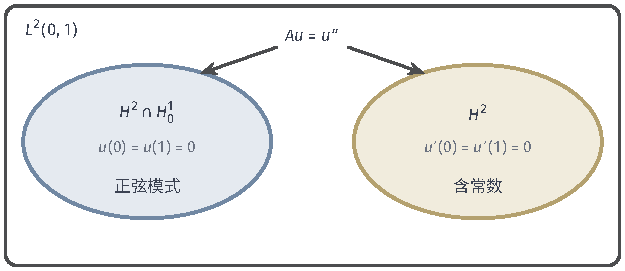
\includegraphics[width=105mm]{figures/06-differential-equations/02-partial-differential-equations/tikz/heat-generator-domain/figure.pdf}
  \caption{同一个表达式$Au=u''$的两个定义域，都是$L^2(0,1)$的稠密子空间。左（蓝）是零Dirichlet条件，由正弦模式张成；右（黄）是零Neumann条件，包含常数，生成不同的半群。}
  \label{fig:heat-generator-domain}
\end{BookInlineFigure}

生成元是无界算子：$\lVert Ae_k\rVert_2=k^2\pi^2\to\infty$，这也是$\lVert S(t)-I\rVert$不趋于零的原因。于是$\mathrm{e}^{tA}$不能用幂级数定义，一般的$u\in L^2$根本不在$D(A^n)$中。空间离散后，这种无界性表现为矩阵最大特征值随网格加细而增长，约为$4/h^2$，图~\ref{fig:heat-unbounded-generator}(b)。

\begin{BookInlineFigure}
  \centering
  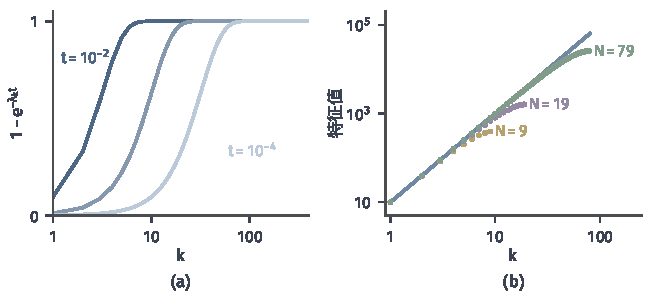
\includegraphics[width=112mm]{figures/06-differential-equations/02-partial-differential-equations/matplotlib/heat-unbounded-generator/figure.pdf}
  \caption{生成元的无界性。(a)$1-\mathrm{e}^{-\lambda_kt}$对$k$的关系，$t=10^{-2},10^{-3},10^{-4}$（蓝色由深到浅），对每个$t$都随$k$增大趋于$1$。(b)离散Laplace矩阵的特征值$4h^{-2}\sin^2(k\pi h/2)$，$N=9,19,79$（点），蓝线是$\lambda_k=k^2\pi^2$，网格越细能到达的特征值越大。}
  \label{fig:heat-unbounded-generator}
\end{BookInlineFigure}

\paragraph{一般区域与源项}
一般的有界区域上，可以用第~\ref{chap:elliptic-equations}章的双线性型定义生成元。令
\[
 a(u,v)=\int_\Omega\nabla u\cdot\nabla v\,\mathrm{d}\bm{x} .
\]
$D(A)$由这样的$u\in H^1_0(\Omega)$组成：存在$g\in L^2(\Omega)$，使$a(u,v)=-\langle g,v\rangle$对所有$v\in H^1_0(\Omega)$成立，此时$Au=g$。Dirichlet边界藏在空间$H^1_0$里，$g$是弱意义下的$\Delta u$。

$-A$的逆是椭圆问题的解算子，它在$L^2(\Omega)$上紧且自伴。由紧自伴算子的谱定理，存在$L^2(\Omega)$的标准正交基$\{e_k\}$和$0<\lambda_1\leq\lambda_2\leq\cdots\to\infty$，于是半群可以直接写成
\begin{equation}
 S(t)u_0=\sum_k\mathrm{e}^{-\lambda_kt}\langle u_0,e_k\rangle e_k ,
 \label{eq:heat-spectral-semigroup}
\end{equation}
谱定理可参考\BookChapterRef{chap:operator-spectra}{卷四第18章“算子谱”}。一般的算子何时生成半群由Hille--Yosida定理回答，它的证明需要预解式的估计，这里的算子已经有了显式的谱表示，所以用不到它。

源项的公式回到前面的切片思想。设$f:[0,T]\to X$连续，
\begin{equation}
 u(t)=S(t)u_0+\int_0^tS(t-s)f(s)\,\mathrm{d}s
 \label{eq:heat-mild}
\end{equation}
称为\term{温和解}（mild solution）。它只要求半群存在，而不要求$u$可微。强连续性和$\lVert S(t)\rVert\leq1$保证被积函数连续，积分在$X$中存在。数据足够好时，它与经典解一致，式~\eqref{eq:heat-duhamel-space}和式~\eqref{eq:heat-duhamel-modes}是它的两个具体形式。

最后，半群和椭圆问题之间有一个简单的关系。在零Dirichlet的情形下，把式~\eqref{eq:heat-spectral-semigroup}对时间从$0$积到$\infty$，每个模式的因子积分为$1/\lambda_k$，所以对$f\in L^2(\Omega)$，
\[
 \int_0^\infty S(t)f\,\mathrm{d}t=(-A)^{-1}f .
\]
恒定热源在无穷长时间内累积的响应，就是Poisson问题的解。例~\ref{ex:heat-source-steady}中$a_k\to f_k/\lambda_k$是这个等式的坐标形式。

与矩阵的对照见表~\ref{tab:heat-matrix-analogy}。

\begin{BookInlineTable}
  \centering
  \caption{矩阵指数与热半群的对照。}
  \label{tab:heat-matrix-analogy}
  \begin{tabular}{lll}
    \toprule
    & 线性常微分方程 & 热方程\\
    \midrule
    演化算子 & $\mathrm{e}^{t\bm{A}}$，$t\in\mathbb{R}$ & $S(t)$，$t\geq0$\\
    生成元 & 有界，处处有定义 & 无界，定义域含边界条件\\
    小时间连续 & 按算子范数 & 只按每个初值\\
    输入响应 & 常数变易公式 & Duhamel公式（温和解）\\
    \bottomrule
  \end{tabular}
\end{BookInlineTable}


\section{逆热问题}
\label{sec:heat-inverse}

设想测得了棒在时刻$T$的温度，想知道时刻$0$的温度。这称为\term{逆热问题}（backward heat problem）。方程本身可逆吗？正向问题适定，反向问题是否同样？

\paragraph{高频被放大}
在$(0,1)$上取零边值，$u(\cdot,T)$的坐标是$y_k=\mathrm{e}^{-\lambda_kT}c_k$。形式上，初值的坐标由$c_k=\mathrm{e}^{\lambda_kT}y_k$恢复，这一步把每个坐标放大$\mathrm{e}^{\lambda_kT}$倍。$T=0.05$时，
\[
 \mathrm{e}^{\lambda_1T}\approx1.64,\quad \mathrm{e}^{\lambda_3T}\approx84.9,\quad \mathrm{e}^{\lambda_5T}\approx2.3\times10^{5},\quad \mathrm{e}^{\lambda_7T}\approx3.2\times10^{10} .
\]
测量总有误差。正向传播把高频压没了，反向传播要把它放大回来，噪声也跟着放大。

图~\ref{fig:heat-inverse-amplify}(b)、(c)显示了问题的另一面：两个明显不同的初值，到$T=0.05$时几乎无法区分。差的部分是$0.12\sin(11\pi x)$，放大因子使它在终态只剩约$10^{-27}$，任何测量都看不出来。

\begin{BookInlineFigure}
  \centering
  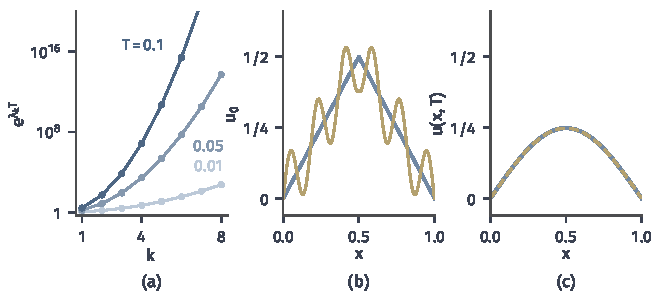
\includegraphics[width=112mm]{figures/06-differential-equations/02-partial-differential-equations/matplotlib/heat-inverse-amplify/figure.pdf}
  \caption{反向恢复的困难。(a)放大因子$\mathrm{e}^{\lambda_kT}$，$T=0.01,0.05,0.1$（蓝色由浅到深），纵轴为对数。(b)三角形初值（蓝）及加上$0.12\sin(11\pi x)$的初值（黄）。(c)二者在$T=0.05$时的解，两条曲线重合。}
  \label{fig:heat-inverse-amplify}
\end{BookInlineFigure}

\paragraph{不适定性}
正向映射是单射，所以终态确实决定初态。可是Hadamard的三条要求中，存在性和连续依赖都失败，这就是\term{不适定问题}（ill-posed problem）的情形。

\begin{theorem}[逆热问题的不适定性]
\label{thm:heat-inverse-illposed}
设$S(T):L^2(0,1)\to L^2(0,1)$是零Dirichlet条件的解算子，$T>0$。
\begin{enumerate}
 \item $S(T)$是单射；$y=\sum_ky_ke_k$属于其值域，当且仅当
 \begin{equation}
  \sum_k\mathrm{e}^{2\lambda_kT}y_k^2<\infty .
  \label{eq:heat-inverse-range}
 \end{equation}
 \item 逆映射不连续：存在$\lVert\eta_n\rVert_2\to0$的扰动，使$\lVert S(T)^{-1}\eta_n\rVert_2\to\infty$。
\end{enumerate}
\end{theorem}

\begin{proof}
(1)若$S(T)u_0=0$，则$\mathrm{e}^{-\lambda_kT}c_k=0$，所以全部$c_k=0$。$y=S(T)u_0$当且仅当$c_k=\mathrm{e}^{\lambda_kT}y_k$平方可和，这就是式~\eqref{eq:heat-inverse-range}。

(2)取$\eta_n=\mathrm{e}^{-\lambda_nT/2}e_n$。它的范数$\mathrm{e}^{-\lambda_nT/2}\to0$。而
\[
 S(T)^{-1}\eta_n=\mathrm{e}^{\lambda_nT/2}e_n,
\]
范数趋于无穷。
\end{proof}

式~\eqref{eq:heat-inverse-range}说，只有极其光滑的函数才是可能的终态。一个带噪声的观测几乎一定不满足它，形式公式的级数发散。

\paragraph{中间时刻的稳定性}
恢复$t=0$是不可能稳定的，但恢复稍早的时刻$0<t<T$好得多，只要预先知道初值有界。由Hölder不等式，取指数$T/(T-t)$与$T/t$，把$c_k^2\mathrm{e}^{-2\lambda_kt}$写成$(c_k^2)^{1-t/T}(c_k^2\mathrm{e}^{-2\lambda_kT})^{t/T}$，
\begin{equation}
 \lVert u(\cdot,t)\rVert_2\leq\lVert u_0\rVert_2^{\,1-t/T}\,\lVert u(\cdot,T)\rVert_2^{\,t/T} .
 \label{eq:heat-log-convexity}
\end{equation}
如果$\lVert u_0\rVert_2\leq R$，两个候选解的差也满足这个不等式，所以观测误差$\delta$在时刻$t$产生至多$(2R)^{1-t/T}\delta^{t/T}$的误差。这个指数$t/T$随$t\to0$退化为零，反映出$t=0$处失去稳定性。

\paragraph{用截断恢复}
放弃高频，只恢复可靠的部分。设观测$y=S(T)u_0+\eta$，$\lVert\eta\rVert_2\leq\delta$。截断重建是
\begin{equation}
 u^{N}=\sum_{k\leq N}\mathrm{e}^{\lambda_kT}\langle y,e_k\rangle\,e_k .
 \label{eq:heat-truncated}
\end{equation}

\begin{theorem}[截断重建的误差]
\label{thm:heat-truncation}
若$u_0\in H^1_0(0,1)$，$\lVert u_0'\rVert_2\leq R$，则
\begin{equation}
 \lVert u^{N}-u_0\rVert_2\leq\mathrm{e}^{\lambda_NT}\delta+\frac{R}{\sqrt{\lambda_{N+1}}} .
 \label{eq:heat-truncation-error}
\end{equation}
\end{theorem}

\begin{proof}
观测的坐标是衰减后的真值加噪声的坐标，代入式~\eqref{eq:heat-truncated}，
\[
 u^{N}-u_0=\sum_{k\leq N}\mathrm{e}^{\lambda_kT}\langle\eta,e_k\rangle e_k-\sum_{k>N}c_ke_k .
\]
第一个和的范数不超过$\mathrm{e}^{\lambda_NT}\delta$，因为每个放大因子不超过$\mathrm{e}^{\lambda_NT}$。第二个和的平方范数是$\sum_{k>N}c_k^2$，由定理~\ref{thm:heat-series}证明中的分部积分和Parseval等式，$\sum_k\lambda_kc_k^2$等于$\lVert u_0'\rVert_2^2$，不超过$R^2$，于是
\[
 \sum_{k>N}c_k^2\leq\frac{1}{\lambda_{N+1}}\sum_{k>N}\lambda_kc_k^2\leq\frac{R^2}{\lambda_{N+1}} .
\]
\end{proof}

误差分成两半：噪声放大随$N$指数增长，截断偏差随$N$缓慢下降。使两者平衡，大致要求$\mathrm{e}^{\lambda_NT}\delta\sim1$，即
\begin{equation}
 N\approx\frac{1}{\pi}\sqrt{\frac{\ln(1/\delta)}{T}} .
 \label{eq:heat-recoverable-scale}
\end{equation}
这个数决定了可恢复的最细尺度。$T=0.05$时，$\delta=10^{-3},10^{-6},10^{-12}$对应$N\approx3.7,\,5.3,\,7.5$。测量精度提高到平方，可恢复的频率只增加到$\sqrt2$倍；相应的偏差只按$1/\sqrt{\ln(1/\delta)}$下降。

\begin{example}[三角形的重建]
\label{ex:heat-inverse-tent}
取三角形初值，$T=0.05$，每个奇数模式的观测都有固定误差$\eta_k=10^{-3}$。第$k$个模式的恢复误差是$10^{-3}\mathrm{e}^{\lambda_kT}$，$k=1,3,5$时分别为$0.0016$、$0.0849$、$228$。而真实系数只有$c_1\approx0.2866$，$c_3\approx-0.0318$，$c_5\approx0.0115$：$k=3$的恢复误差已经比系数本身大，$k=5$则完全被噪声淹没。总误差如表~\ref{tab:heat-inverse-error}，最好的选择是只保留$k=1$。
\end{example}

\begin{BookInlineTable}
  \centering
  \caption{三角形初值的截断重建误差，$T=0.05$，每个奇数模式的观测误差为$10^{-3}$，取$k\leq N$的奇数模式。}
  \label{tab:heat-inverse-error}
  \begin{tabular}{llll}
    \toprule
    $N$ & 噪声放大 & 截断偏差 & $L^2$总误差\\
    \midrule
    $1$ & $0.0016$ & $0.0347$ & $0.0348$\\
    $3$ & $0.0849$ & $0.0138$ & $0.0860$\\
    $5$ & $228$ & $0.0078$ & $228$\\
    \bottomrule
  \end{tabular}
\end{BookInlineTable}

图~\ref{fig:heat-inverse-recon}画出了这三种重建。$N=1$时得到一条平滑的拱形，整体位置正确；$N=3$时噪声开始主导；$N=5$时重建的幅度达到数百，已经和三角形毫无关系。

\begin{BookInlineFigure}
  \centering
  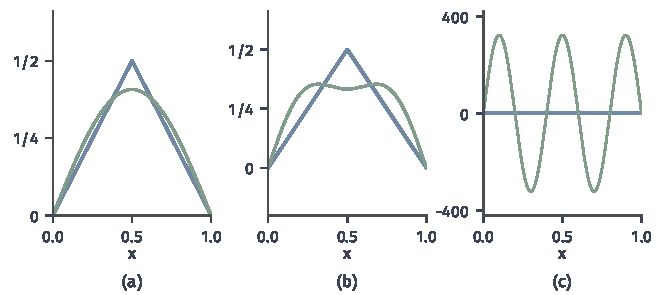
\includegraphics[width=112mm]{figures/06-differential-equations/02-partial-differential-equations/matplotlib/heat-inverse-recon/figure.pdf}
  \caption{截断重建，$T=0.05$，每个奇数模式的观测误差为$10^{-3}$。蓝线是真实的三角形，绿线是$u^{N}$。(a)$N=1$。(b)$N=3$。(c)$N=5$，注意纵轴范围。}
  \label{fig:heat-inverse-recon}
\end{BookInlineFigure}

\paragraph{Tikhonov滤波}
截断是硬开关。\term{Tikhonov正则化}（Tikhonov regularization）用平滑的滤波代替它。设$\sigma_k=\mathrm{e}^{-\lambda_kT}$，取$\alpha>0$，极小化
\[
 \lVert S(T)v-y\rVert_2^2+\alpha\lVert v\rVert_2^2 .
\]
这个问题按坐标分开，第$k$个坐标是一元二次函数，解为
\begin{equation}
 v_k=\frac{\sigma_k}{\sigma_k^2+\alpha}\,y_k .
 \label{eq:heat-tikhonov}
\end{equation}
增益$\sigma/(\sigma^2+\alpha)$在$\sigma=\sqrt\alpha$处最大，最大值是$1/(2\sqrt\alpha)$，所以噪声放大不超过这个数。$\sigma\gg\sqrt\alpha$的低频几乎按$1/\sigma$恢复，$\sigma\ll\sqrt\alpha$的高频被压到零。

取$\alpha=10^{-4}$，增益的上限是$50$。$T=0.05$时，$k=1,3,5$的增益分别是$1.64$、$49.3$、$0.044$，未正则化时是$1.64$、$84.9$、$2.3\times10^5$。图~\ref{fig:heat-inverse-tradeoff}(a)是不同噪声水平下总误差随$N$的变化，呈现先降后升的形状；图~\ref{fig:heat-inverse-tradeoff}(b)比较了三种增益。

\begin{BookInlineFigure}
  \centering
  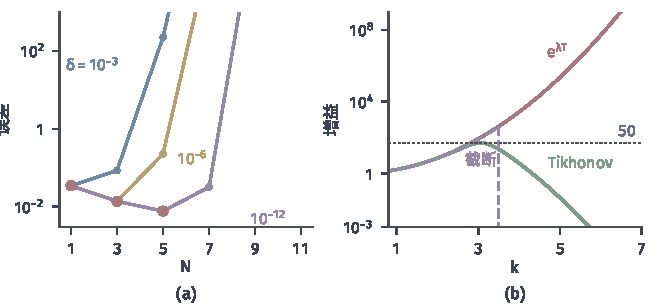
\includegraphics[width=112mm]{figures/06-differential-equations/02-partial-differential-equations/matplotlib/heat-inverse-tradeoff/figure.pdf}
  \caption{噪声与可恢复尺度。(a)三角形初值，$T=0.05$，每个奇数模式的观测误差$\delta=10^{-3},10^{-6},10^{-12}$时$L^2$总误差随$N$的变化，红点是最优的$N$。(b)作为连续变量$k$的增益：未正则化的$\mathrm{e}^{\lambda T}$（红）、截断（紫色虚线，示意取在$k=3.5$）、$\alpha=10^{-4}$的Tikhonov滤波（绿），点线是增益上限$50$。}
  \label{fig:heat-inverse-tradeoff}
\end{BookInlineFigure}

正则化并不能恢复已经丢失的信息，它只是诚实地放弃了高频，用先验（如初值的范数有界）换取稳定。正向过程越能抹平细节，反向过程就越难找回细节，这两者是同一个衰减因子的两面。


\section{本章小结}
\label{sec:heat-summary}

本章回答了一个局部规律怎样决定整体演化的问题。每一点向邻居的平均值靠拢，写成方程是$\partial_tu=\Delta u+f$，再加上一个初值和边界条件，问题就确定了。固定温度和无通量是两种不同的物理规定，前者让热量流出，后者保留一个零模式。

同一个传播过程有四种描述，它们各有适用的场合，见表~\ref{tab:heat-summary}。边界模式把问题对角化，高频衰减得快，零模式不衰减；热核把一点的影响写成Gauss钟形，宽度按$\sqrt{t}$增长；能量和极值估计不需要显式公式；半群把解看成算子，边界条件落在生成元的定义域中。

\begin{BookInlineTable}
  \centering
  \caption{同一扩散过程的四种描述。}
  \label{tab:heat-summary}
  \begin{tabular}{lll}
    \toprule
    描述 & 适用情形 & 看到的结构\\
    \midrule
    边界模式 & 有界区域，零边值 & 独立模式按$\mathrm{e}^{-\lambda_kt}$衰减\\
    热核卷积 & 全空间，受增长限制 & Gauss平均，$\sqrt{t}$尺度\\
    能量与极值 & 一般区域，明确的边界 & 耗散、比较、唯一性\\
    解半群 & 选定函数空间 & 时间拼接，无界生成元\\
    \bottomrule
  \end{tabular}
\end{BookInlineTable}

结论的成立范围都有明确的边界。初值恢复的方式取决于数据：有界一致连续初值一致恢复，$L^p$初值（$1\leq p<\infty$）在$L^p$中恢复，一般$L^\infty$初值只在连续点逐点恢复。全空间的唯一性要限制增长，否则有Tikhonov解。经典解的公式需要相应的正则性和相容性，粗糙数据时只能在$L^2$或弱的意义下理解。估计都是有限时间的，长期行为的一般理论不在本卷。

持续输入和非齐次边界都归结到同一条原则：线性叠加，把输入切片后逐片自由演化。这个原则要求已经知道自由演化；非零边值要先提升，全空间卷积不能直接用于有界区域。

平滑效应是扩散最突出的特点，也是逆问题困难的根源。正向过程在$t>0$时把高频按指数压低，反向恢复必须把它们放大回来，所以可恢复的频率只随测量精度的对数增长。

第~\ref{chap:wave-equations}章的波动方程有两个初值、有限的传播速度和守恒的能量，可以与这里的耗散和瞬间影响逐条比较。随机路径、转移概率和Fokker--Planck方程给出的概率解释不属于本卷范围，空间离散则在第~\ref{chap:pde-numerical-methods}章讨论。

